\documentclass[onecolumn, compsoc,10pt]{IEEEtran}
\let\labelindent\relax
\usepackage{enumitem}
\input{preamble.tex}  
\def\V{\mathds{V}}
\def\Appendix{Appendix}
%###################################

\newif\iftikzX
\tikzXtrue
\tikzXfalse
%--------------
\def\jobnameX{zero}
%--------------
\newif\ifFIGS
\FIGSfalse 
\FIGStrue
%--------------
\newif\ifdraftQ
\draftQtrue
%\draftQfalse
%--------------
%###################################
\def\TITLE{\enet: Fast Scalable Pandemic Risk Assessment of \infl Strains Circulating In Non-human Hosts}
%\def\TITLE{\LARGE A Biologically Meaningful Sequence Metric\\For Analyzing Evolutionary Changes\\In Novel Pathogens}
%\def\TITLE{Learning  Mutational Patterns At Scale For\\Analysis Of Sequence Divergence\\In Novel Pathogens}
%\def\TITLE{Learning Mutational Patterns at Scale to Analyze Sequence Divergence in Novel Pathogens}

\def\authore{Kevin Wu}
\def\authora{ Jin Li}
\def\authorc{Aaron Esser-Kahn}
\def\authord{Ishanu Chattopadhyay}

\def\addressa{Department of Medicine, University of Chicago, IL, USA}
\def\addressb{Committee on Genetics, Genomics \& Systems Biology, University of Chicago, IL, USA}
\def\addressc{Committee on Quantitative Methods in Social, Behavioral, and Health Sciences, University of Chicago, IL, USA}
\def\addressd{Pritzker School of Molecular Engineering, University of Chicago, Chicago, IL, USA}
\def\addresse{Committee on Immunology, University of Chicago, Chicago, IL, USA}
\newif\ifdraftQ
\draftQtrue
\draftQfalse


%###################################

\title{\LARGE \TITLE}
\author{\sffamily  \fontsize{10}{12}\selectfont   \authore$^{1}$,\authora$^{1}$,  \authorc$^{2,3}$, and \authord$^{1,4,5\bigstar}$\\                                                                
\vspace{10pt}                                                                   

\sffamily  \fontsize{10}{12}\selectfont                                         
$^{1}$\addressa\\   
$^{2}$\addressd\\
$^{3}$\addresse\\
$^{5}$\addressc                                                                 
\vskip 1em                                                                      
$^\bigstar$To whom correspondence should be addressed: e-mail: \texttt{ishanu@uchicago.edu}.}


\def\hcov{SARS-CoV-2\xspace}
\def\RATG13{RaTG13\xspace}
\def\Appendix{Appendix}
\def\qnet{Enet\xspace}
\def\enet{Emergenet\xspace}
\def\erisk{E-risk\xspace}
\def\qdist{E-distance\xspace}
\def\cov{COVID-19\xspace}
\def\infl{Influenza A\xspace}
%\def\infl{IAV\xspace}


\def\E{\mathcal{E}}
\def\dst{x_\star^{t+\delta}}
\def\dsta{x^{t+\delta}}
 
\usepackage{flushend}
%\externaldocument[SI-]{SI}
% \externaldocument[EXT-]{exfig}
\newif\iftikzX
\tikzXtrue
\tikzXfalse
\def\EXTENDED{Extended Data\xspace}
\def\SUPPLEMENTARY{Supplementary\xspace}
\newif\ifFIGS
\FIGSfalse  
\FIGStrue 

\def\METHODS{Online Methods\xspace}

  
\tikzexternalenable    
%\pgfplotsset{compat=1.18}

\begin{document}  
\maketitle  

{\bf \sffamily \fontsize{10}{12}\selectfont \noindent   
  {\normalfont \itshape Abstract:} Animal influenza  viruses emerging into humans % are suspected to
  have triggered devastating  pandemics in the past~\cite{shao2017evolution,mills2004transmissibility,reid2003origin,landolt2007up}. Yet, our ability to evaluate the pandemic potential of individual strains that do not yet circulate in humans, remains limited. In this study we introduce the \enet (Enet), to computationally learn how new variants emerge, shaped by evolutionary constraints using only observed genomic sequences  of key viral proteins. Analyzing Haemagglutinnin (HA) and Neuraminidase (NA) sequences from $>159,000$ sequenced strains, we estimate the likelihood of specific future mutations, and the numerical odds of  specific descendants arising via natural processes. After validating our model to forecast the dominant strain(s) for seasonal flu, with \enet-based forecasts significantly outperforming WHO recommendations almost consistently over the past two decades for H1N1/H3N2 subtypes, individually in the Northern/Southern hemispheres (average match-improvement $32.25\% $ over two decades, $69.07\%$ over the last decade, and $81.13\%$ over the pre-\cov five year period for H1N1 HA), we assess the pandemic potential of animal strains not yet known to transmit in humans. While the state-of-the-art Influenza Risk Assessment Tool (IRAT) from the CDC to assess such risk includes time-consuming experimental assays, our calculations take $\approx 6s/$strain, yet strongly correlating with published IRAT scores (correlation$: 0.703$, p-value$: 0.00026$). This six orders of magnitude speedup is  necessary to exploit  current surveillance capacity via scalably analyzing thousands of strains collected annually. Considering $6,066$ wild \infl viruses sequenced post-2020, we identify risky strains of diverse subtypes, hosts and geo-locations, with six having estimated emergence scores $> 6.5$. Such scalable risk-ranking can enable preemptive pandemic mitigation, including the targeted inoculation of animal hosts before the first human infection, and outline new public health measures that are potentially effective notwithstanding possible vaccine hesitancy in humans.}
  
\vspace{10pt} 

\subsection*{Introduction}
Influenza viruses constantly evolve~\cite{dos2016influenza}, sufficiently altering surface protein structures to evade the prevailing host immunity, and cause the recurring seasonal  epidemic. These periodic  infection peaks claim a quarter to half a million lives~\cite{huddleston2020integrating} globally,  and currently our response hinges on annually  inoculating  the  human population with a  reformulated  vaccine~\cite{boni2008vaccination,dos2016influenza}.  Among numerous factors that hinder optimal design of the flu shot, failing to correctly predict the future dominant strain  dramatically reduces vaccine effectiveness~\cite{tricco2013comparing}. Despite  recent advances~\cite{neher2014predicting,huddleston2020integrating} such predictions remain imperfect. In addition to  the seasonal  epidemic, influenza strains spilling over into humans from animal reservoirs have triggered  pandemics  at least four times (1918 Spanish flu/H1N1, 1957 Asian flu/H2N2, 1968 Hong Kong flu/H3N2, 2009 swine flu/H1N1) in the past 100 years~\cite{shao2017evolution}. With the memory of the  sudden \hcov emergence
fresh in our minds, a looming question  is whether we can  preempt and mitigate such events in the future. \infl, partly on account of its segmented genome and its wide prevalence in common animal hosts, can easily incorporate genes from multiple strains and (re)emerge as novel human pathogens~\cite{reid2003origin,vergara2014ns}, thus harboring  a high pandemic potential.

\def\MXCOL{black}
\def\FXCOL{Orchid3}
\def\MNCOL{SeaGreen4}
\def\FNCOL{SeaGreen4}
\def\NCOL{SeaGreen4}
\def\XCOL{Tomato}
\def\WCOL{Tomato}
\def\YCOL{DodgerBlue4}
\def\TEXTCOL{gray}
\def\AXISCOL{white}
%###################################                                            
%###################################                                            
\ifFIGS
\begin{figure*}[!ht]
  \tikzexternalenable
  \tikzsetnextfilename{scheme}
  \centering
 %\tikzXtrue
  \iftikzX  
  \def\EPATH{e2}
  \begin{tikzpicture}[font=\bf\sffamily\fontsize{8}{9}\selectfont]
  \def\DCOL{Tomato}
  \def\DCOLx{Tomato}
  \def\DCOL{black!50}
  \def\DCOLx{black!80}
  \def\DCOLS{black}
  \def\ECOLA{black!5}
  \def\ECOLB{black!5}
  \def\ECOLC{Green4!5}
  \def\ECOLD{Green4!5}
  \def\LWD{1pt}
  \def\LWDA{6pt}
  \def\ACOL{black}
  \def\OPC{.8}
  \def\OPCA{.95}
  \def\OPCB{.15}
  \def\CIRC{circle}
  \def\LWT{2pt}
  \def\SCALE{.80}
  \def\LCOL{black!50}
  \node[anchor=south west] (T) at (0,0) {
    \includegraphics[width=3in]{Figures/\EPATH}};

  \node[anchor=south west,label={[text=black,align=center,yshift=-0in,xshift=2.25in]120:{\Large b.} A sample of conditional inference trees\\in inferred \enet (H1N1 HA)}] at ([yshift=0in]T.south east) {
    \begin{tikzpicture}[anchor=center,font=\bf\sffamily\fontsize{8}{8}\selectfont]
      \clip (.93in,-0in) rectangle (-2.85in,-7in);
      \tikzset{xcirc/.style={circle,inner sep=-25pt,dashed,fill=\ECOLB,opacity=\OPC,rounded corners=5pt,draw=\DCOL,line width=\LWD,scale=\SCALE}}
      \def\WDT{2.5in}
      \def\WDTA{2.25in}
      \def\WDTB{2in}
      \def\WDTC{2.40in}
      \coordinate (Z) at (0,0);

      \node[anchor=north west,xcirc,inner sep=-35pt,label={[yshift=.9in,xshift=-.5in,align=center,\LCOL]-90:index\\63}] (P63) at ([xshift=-2.9in,yshift=-.75in]Z) {\includegraphics[width=\WDTB]{../qnet_predictions/qnet_models/trees/proc63}}; 

      
      \node[anchor=north,xcirc,inner sep=-20pt,label={[xshift=-.6in,yshift=.7in,align=center,\LCOL]-90:index\\155}] (P155) at (Z) {\includegraphics[width=\WDTC]{../qnet_predictions/qnet_models/trees/proc155}};

      \node[anchor=north,xcirc,inner sep=-25pt,label={[yshift=.65in,xshift=-.45in,align=center,\LCOL]-90:index\\14}] (P14) at ([xshift=-2.2in,yshift=-0.8in]P155.south) {\includegraphics[width=\WDTB]{../qnet_predictions/qnet_models/trees/proc14}}; 
      
      \node[anchor=north,xcirc,inner sep=-25pt,label={[yshift=.6in,xshift=-.5in,align=center,\LCOL]-90:index\\223}] (P223) at ([xshift=-0in,yshift=-0.10in]P155.south) {\includegraphics[width=\WDT]{../qnet_predictions/qnet_models/trees/proc223}};


      \node[text width=.13in,  rounded corners=8pt, line width=2pt,,inner sep=10pt,opacity=1,draw=\DCOLx] (X1) at ([yshift=.835in,xshift=.12in]P63) {};
      \draw [line width=\LWT,\DCOLx,-latex,] (X1)  to [out=75,in=140,looseness=1.55]  (P155);

      \node[text width=.13in,  rounded corners=8pt, line width=2pt,inner sep=10pt,opacity=1,draw=\DCOLx] (X2) at ([yshift=.845in,xshift=-.335in]P155) {};
      \draw [line width=\LWT,\DCOLx,-latex,] (X2)  to [out=0,in=60,looseness=1]  (P223);

      \node[text width=.13in,  rounded corners=8pt, line width=2pt,,inner sep=10pt,opacity=1,draw=\DCOLx] (X3) at ([yshift=.0in,xshift=.12in]P14) {};
      \draw [line width=\LWT,\DCOLx,-latex,] (X3)  to [out=150,in=-120,looseness=1.1]  (P63);

      \node[text width=.15in,  rounded corners=8pt, line width=2pt,inner sep=10pt,opacity=1,draw=\DCOLx] (X4) at ([yshift=.88in,xshift=-.34in]P223) {};
      \draw [line width=\LWT,\DCOLx,-latex,] (X4)  to [out=210,in=35,looseness=1.2]  (P14);

      \node[anchor=north,align=left,font=\bf\tt\footnotesize] (N3) at ([yshift=-6.1in,xshift=-1.85in]Z.south) {\bf\sffamily\fontsize{7}{8}\selectfont H1N1 2020-2021\\\bf\sffamily\fontsize{7}{8}\selectfont Haemagglutinin Sequences\\$\cdots$GTSRY{\color{Red1}S}KKFKPEIATRPKVRDQEGR$\cdots$\\$\cdots$GTSKY{\color{Red1}G}KKFMPEIARRPKVRNQEGR$\cdots$\\
        $\cdots$GSSKY{\color{Red1}Y}KRFTPEIVARPKVREQAGR$\cdots$\\
 $\cdots$GSSKY{\color{Red1}Y}KRFTPEIVARPKVREQAGR$\cdots$};

%A/Niger/8327/2020 
%
%A/Parana/10835/2021
%A/Gansu-Xifeng/1143/2021
%A/Sichuan/01208/2021

   \node[anchor=west,align=left,font=\bf\sffamily\fontsize{8}{10}\selectfont] (N4) at ([xshift=0.1in,yshift=.05in]N3.east) {A/Niger/8327/2020 \\
    A/Parana/10835/2021\\
      A/Gansu-Xifeng/1143/2021\\  
      A/Sichuan/01208/2021};

       \draw [ultra thick] ([yshift=.25in,xshift=.01in]N4.west) --++ (-.13in,-.190in);
       \draw [ultra thick] ([yshift=.1in,xshift=.01in]N4.west) --++ (-.13in,-.2in);
       \draw [ultra thick] ([yshift=-0.05in,xshift=.01in]N4.west) --++ (-.13in,-.2in);
       \draw [ultra thick] ([yshift=-.2in,xshift=.01in]N4.west) --++ (-.13in,-.2in);

       \node [align=center,text=IndianRed2,anchor=north] at ([xshift=-2.25in,yshift=-.1in]N4.south) {index 223};

      \node[anchor=west,rounded corners=3pt,align=center] (I1) at ([yshift=-.6in,xshift=.3in]P14.south west) {Color key (mixed colors represent distributions)};


      \definecolor{Acol}{RGB}{255,193,85}
      \definecolor{Dcol}{RGB}{255,255,85}
      \definecolor{Ecol}{RGB}{255,255,85}
      \definecolor{Gcol}{RGB}{136,255,85}
      \definecolor{Icol}{RGB}{85,255,150}
      \definecolor{Kcol}{RGB}{85,255,255}
      \definecolor{Lcol}{RGB}{85,255,255}
      \definecolor{Qcol}{RGB}{111,85,255}
      \definecolor{Scol}{RGB}{231,85,255}
      \definecolor{Tcol}{RGB}{255,85,255}
      \definecolor{Vcol}{RGB}{255,85,255}
      \definecolor{Ycol}{RGB}{255,85,97}
      
      \node[font=\bf\sffamily,anchor=north,rounded corners=3pt,text width=.1in,text height=.1in,fill=Acol,align=center,opacity=\OPC] (I1) at ([yshift=-.05in]I1.south west) {A};
      \node[font=\bf\sffamily,anchor=west,rounded corners=3pt,text width=.1in,text height=.1in,fill=Dcol,align=center,opacity=\OPC] (I1) at ([xshift=.05in]I1.east) {D};
      \node[font=\bf\sffamily,anchor=west,rounded corners=3pt,text width=.1in,text height=.1in,fill=Ecol,align=center,opacity=\OPC] (I1) at ([xshift=.05in]I1.east) {E};
      \node[font=\bf\sffamily,anchor=west,rounded corners=3pt,text width=.1in,text height=.1in,fill=Gcol,align=center,opacity=\OPC] (I1) at ([xshift=.05in]I1.east) {G};
      \node[font=\bf\sffamily,anchor=west,rounded corners=3pt,text width=.1in,text height=.1in,fill=Icol,align=center,opacity=\OPC] (I1) at ([xshift=.05in]I1.east) {I};
      \node[font=\bf\sffamily,anchor=west,rounded corners=3pt,text width=.1in,text height=.1in,fill=Kcol,align=center,opacity=\OPC] (I1) at ([xshift=.05in]I1.east) {K};
      \node[font=\bf\sffamily,anchor=west,rounded corners=3pt,text width=.1in,text height=.1in,fill=Lcol,align=center,opacity=\OPC] (I1) at ([xshift=.05in]I1.east) {L};
      \node[font=\bf\sffamily,anchor=west,rounded corners=3pt,text width=.1in,text height=.1in,fill=Qcol,align=center,opacity=\OPC] (I1) at ([xshift=.05in]I1.east) {Q};
      \node[font=\bf\sffamily,anchor=west,rounded corners=3pt,text width=.1in,text height=.1in,fill=Scol,align=center,opacity=\OPC] (I1) at ([xshift=.05in]I1.east) {S};
      \node[font=\bf\sffamily,anchor=west,rounded corners=3pt,text width=.1in,text height=.1in,fill=Tcol,align=center,opacity=\OPC] (I1) at ([xshift=.05in]I1.east) {T};
      \node[font=\bf\sffamily,anchor=west,rounded corners=3pt,text width=.1in,text height=.1in,fill=Vcol,align=center,opacity=\OPC] (I1) at ([xshift=.05in]I1.east) {V};
      \node[font=\bf\sffamily,anchor=west,rounded corners=3pt,text width=.1in,text height=.1in,fill=Ycol,align=center,opacity=\OPC] (I1) at ([xshift=.05in]I1.east) {Y};

      % \node[font=\bf\sffamily,anchor=north,rounded corners=3pt,text width=.1in,text height=.1in,fill=DarkOrange3!70,align=center,opacity=\OPC] (I1) at ([yshift=-.05in]I1.south) {A};

      % \node[font=\bf\sffamily,anchor=north,rounded corners=3pt,text width=.1in,text height=.1in,fill=SeaGreen2,align=center,opacity=\OPC] (I1) at ([yshift=-.05in]I1.south) {C};

      % \node[font=\bf\sffamily,anchor=north,rounded corners=3pt,text width=.1in,text height=.1in,fill=DodgerBlue2!80,align=center,opacity=\OPC] (I1) at ([yshift=-.050in]I1.south) {G};
    \end{tikzpicture}
  };

  \node [anchor=south west] (L1) at ([yshift=-.2650in]T.north west) {\Large a.};
  \node [anchor=south west] (L2) at ([yshift=-3.25in]T.north west) {\Large c.};
  \node [anchor=south west] (L3) at ([yshift=-5.65in]T.north west) {\Large d.};

\end{tikzpicture}

 \else
  \includegraphics[width=\textwidth]{Figures/External/scheme}
  \fi
  \vspace{-20pt}
  
 \captionN{\textbf{\enet inference and applications}. \textbf{a}, Variations of
   genomes for identical subgroups of \infl are analyzed to infer a recursive forest of conditional inference trees~\cite{Hothorn06unbiasedrecursive} -- the \enet --   which maximally captures the emergent  dependencies between an a priori unspecified number of   mutations, deletions and insertions. With these inferred dependencies we can    estimate the numerical odds of specific mutations, and by extension, the numerical value of
   the probability of one strain giving rise to another in the wild, under  complex selection pressures from the background. b, Snapshot of decision trees  from the
   \enet constructed for H1N1 haemagglutinnin 2018 sequences. Note that the decision tree predicting the bases at index 1274   uses the bases at 1064, 1445, 197 as features. These features are automatically selected, as being maximally predictive  of the bases be at 1274. Then, we compute predictors for each of these  feature indices, $e.g.$   trees for  index 1064, which involves index 1314 and 339 as features. Continuing, we find that the trees for index 1314 involves indices 1263, 636 and 21, and that for 1263 involves 1314, 667 and 313. The predictor for 1263  depends on 1314, and that for 1314 depends on 1263, revealing the recursive structure of \enet. c, First application: With \enet induced ability to quantify mutation probabilities,  we forecast  dominant strain(s) for the next flu season, using only  sequences collected in the previous season (and the inferred \enet, using data from the past year). d, Second application: estimation of the risk of a global pandemic posed by individual animal strains that are still not known to circulate in humans.}\label{figscheme}.
\end{figure*}
\else
\refstepcounter{figure}\label{figscheme}
\fi  
%#############################################                                  
%#############################################                                  
%#############################################
%#############################################
\ifFIGS
\begin{figure*}[!ht]
  \centering
  \tikzexternalenable
   \tikzsetnextfilename{seasonalpred_both}

  \tikzXtrue 
  \iftikzX
  \hspace{-20pt}\resizebox{.975\linewidth}{!}{\begin{tikzpicture}
  \def\HGT{.35in}
  \def\WDT{2.75in}
  \def\YST{-.3in}

  \node[,label={[font=\bf\sffamily,yshift=-.60in]90:\underline{Southern Hemisphere (Prediction in December)}}] (AAA) at (0,0) {\input{Figures/seasonalpred_southern.tex}};
  \node[anchor=north,label={[font=\bf\sffamily]90:\underline{Northern Hemisphere (Prediction in February)}}] (BBB) at ([yshift=-.25in]AAA.south) {\pgfplotsset{
  discard if/.style 2 args={
    x filter/.append code={
      \edef\tempa{\thisrow{#1}}
      \edef\tempb{#2}
      \ifx\tempa\tempb
      \def\pgfmathresult{inf}
      \fi
    }
  },
  discard if not/.style 2 args={
    x filter/.append code={
      \edef\tempa{\thisrow{#1}}
      \edef\tempb{#2}
      \ifx\tempa\tempb
      \else
      \def\pgfmathresult{inf}
      \fi
    }
  }
}

\begin{tikzpicture}

  \def\NNX{1}
  \noexpand\def\YMAX{15}
  \def\YLABEL{}
  \newcommand{\PPX}[3][2001]{
    \begin{axis}[name=XX,\TEXTCOL,anchor=center,
      title={},legend columns=1,
      legend style={text=black,anchor=west,at={(0.5,1.8)},
        inner sep=1pt,draw=none,fill=black!5,fill opacity=.75,align=right,
        text opacity=1,/tikz/column 2/.style={
          column sep=5pt,
        },},
      ymax=0,
      ymin=-\YMAX,
      xmin=#1,
      xmax=2022,
      name=X0,
      anchor=center,
      width=\WDT,
      height=\HGT,
      scale only axis=true,
      enlargelimits=false,
      enlarge y limits=false,
      enlarge x limits=0.06,
      axis on top=false,
      axis line style={black!2, very thick},
      grid=both,minor x tick num=3,
      major grid style={opacity=1,,thick,black!10},
      minor grid style={opacity=1,,semithick,Red4!5},
      major tick length=0pt,
      minor tick length=0pt,
      ytick style={draw=none},
      scaled y ticks = false,
      y tick label style={/pgf/number format/fixed,
        /pgf/number format/1000 sep = \empty % \thinspace optional
      },
      x tick label style={/pgf/number format/fixed,
        /pgf/number format/1000 sep = \empty % Optional
      },
      xlabel={year},ylabel style={yshift=1in,align=center,xshift=1.9in},
      xlabel style={yshift=.05in},ybar,,bar width=\BWIDTH,
      ytick={#2},%xtick={2000,2004,2008,2012,2016,2020}
      ,xticklabels={},xlabel={},ylabel={\YLABEL},,ylabel style={yshift=-.8in,align=center,xshift=-1.9in},
      xtick=data, xticklabel style={rotate=90}]
      
      \addplot [area legend,restrict x to domain=0:2022,negstyle]
      table [col sep=comma,x expr=\coordindex+#1,
      y expr=(\thisrow{\NMX}
      -\thisrow{ldistance_WHO})/(\NNX)] {\DATAQNETx};
    \end{axis}
    % 
    \begin{axis}[\TEXTCOL,anchor=center,yshift=\HGT,
      title={},legend columns=1,legend style={text=black,anchor=west,at={(0.5,.8)},
        inner sep=1pt,draw=none,fill=black!5,fill opacity=.75,align=right,
        text opacity=1,/tikz/column 2/.style={
          column sep=5pt,
        },},
      ymin=0,
      ymax=\YMAX,
      xmax=2022,
      xmin=#1,
      name=X0,
      anchor=center,
      width=\WDT,
      height=\HGT,
      scale only axis=true,
      enlargelimits=false,
      enlarge y limits=false,
      enlarge x limits=0.06,
      axis on top=false,
      axis line style={black!2, very thick},
      grid=both,minor x tick num=3,
      major grid style={opacity=1,,thick,black!10},
      minor grid style={opacity=1,,semithick,Red4!5},
      major tick length=0pt,
      minor tick length=0pt,
      ytick style={draw=none},
      scaled y ticks = false,
      y tick label style={/pgf/number format/fixed,
        /pgf/number format/1000 sep = \empty % \thinspace optional
      },
      x tick label style={/pgf/number format/fixed,
        /pgf/number format/1000 sep = \empty % Optional
      },
      xlabel={year},ylabel style={yshift=0.8in,align=center,xshift=1in},
      xlabel style={yshift=.05in},ybar,,bar width=\BWIDTH,ytick={#3},,%xtick={2000,2004,2008,2012,2016,2020},
      xticklabels={},xlabel={},xtick=data, xticklabel style={rotate=90}]
      
      \addplot [area legend,restrict x to domain=0:2022,posstyle]
      table [col sep=comma,x expr=\coordindex+#1,y expr=(\thisrow{\NMX}-\thisrow{ldistance_WHO})/(\NNX)] {\DATAQNETx};
    \end{axis}

    \begin{axis}[\TEXTCOL,anchor=center,yshift=0,
      title={},legend columns=1,legend style={text=black,anchor=west,at={(0.5,.8)},
        inner sep=1pt,draw=none,fill=black!5,fill opacity=.75,align=right,
        text opacity=1,/tikz/column 2/.style={
          column sep=5pt,
        },},
      ymin=0,
      ymax=\YMAX,
      xmax=2022, 
      xmin=#1,
      name=X0,
      anchor=center,
      width=\WDT,
      height=\HGT,
      scale only axis=true,
      enlargelimits=false,
      enlarge y limits=false,
      enlarge x limits=0.060,
      axis on top=false,
      axis line style={black!2, very thick},
      % grid,
      grid style={opacity=1,dashed,thick,black!10},
      major tick length=0pt,
      ytick style={draw=none},
      scaled y ticks = false,
      y tick label style={/pgf/number format/fixed,
        /pgf/number format/1000 sep = \empty % \thinspace optional
      },
      x tick label style={/pgf/number format/fixed,
        /pgf/number format/1000 sep = \empty % Optional
      },
      xlabel={year},ylabel style={yshift=0.2in,align=center,xshift=1in},
      xlabel style={yshift=.05in},ybar,
      ,bar width=\BWIDTH,ytick={},yticklabels={},
      %,xtick={2000,2004,2008,2012,2016,2020},
      xlabel={},xtick=data, xticklabel style={rotate=90}]
      
      \addplot [area legend,restrict x to domain=0:2022,draw=none,fill=none]
      table [col sep=comma,x expr=\coordindex+#1,y expr=0] {\DATAQNETx};
    \end{axis}
  }

  \def\TEXTCOL{gray}
  \def\RCLR{IndianRed1}
  \def\RCLRB{IndianRed1}
  \def\QCLRC{Orchid3}
  \def\QCLD{gray!50}
  \def\QCLRB{black}
  \def\QCLR{black}
  \noexpand\def\PCOL{black!0}
  \noexpand\def\NCOL{black!0}
  \noexpand\def\PCOLf{black!90}
  \noexpand\def\NCOLf{Red1}
  \def\SC{1.35}
  \def\XCOL{lightgray!70}
  \def\BWIDTH{8.2pt}
  \tikzset{%
    posstyle/.style =   {line width=1pt,
      draw=\PCOL,fill=\PCOLf}}
  \tikzset{%
    negstyle/.style =   {line width=1pt,
      draw=\NCOL,fill=\NCOLf}}
  %\def\HGT{.3in}
  %\def\WDT{2.75in}
  %\def\YST{-.3in}

  \def\YTICKA{0,-5,-10}
  \def\YTICKB{0,5,10}
  \def\NMX{ldistance_Qnet_recommendation}

  
  \node[anchor=north west] (A) at (0,0) {\begin{tikzpicture}[anchor=center,font=\bf\sffamily\fontsize{8}{9}\selectfont]
      \def\DATAQNETx{Figures/plotdata/north_h1n1_ha.csv}
      \def\YLABEL{}
      \PPX[2002]{\YTICKA}{\YTICKB}
    \end{tikzpicture}};

  \node[anchor=north west] (B) at ([yshift=\YST]A.south west) {\begin{tikzpicture}[anchor=center,font=\bf\sffamily\fontsize{8}{9}\selectfont]
      \def\DATAQNETx{Figures/plotdata/north_h1n1_na.csv}
      \def\YLABEL{}
      \PPX[2002]{\YTICKA}{\YTICKB}
    \end{tikzpicture}};

  \node[anchor=north west] (C) at ([xshift=-.25in,yshift=0in]A.north east) {\begin{tikzpicture}[anchor=center,font=\bf\sffamily\fontsize{8}{9}\selectfont]
      \def\DATAQNETx{Figures/plotdata/north_h3n2_ha.csv}
      \def\YLABEL{}
      \PPX[2006]{\YTICKA}{\YTICKB}
    \end{tikzpicture}};

  \node[anchor=north west] (D) at ($(B.north west)!(C.west)!(B.north east)$) {\begin{tikzpicture}[anchor=center,font=\bf\sffamily\fontsize{8}{9}\selectfont]
      \def\DATAQNETx{Figures/plotdata/north_h3n2_na.csv}
      \def\YLABEL{}
      \PPX[2004]{\YTICKA}{\YTICKB}
    \end{tikzpicture}};

\def\NMX{ldistance_Qnet_recommendation_0}

  \node[anchor=north west] (E) at ([yshift=\YST]B.south west) {\begin{tikzpicture}[anchor=center,font=\bf\sffamily\fontsize{8}{9}\selectfont]
      \def\DATAQNETx{Figures/plotdata/north_h1n1_na_3cluster.csv}
      \def\YLABEL{}
      \PPX[2002]{\YTICKA}{\YTICKB}
    \end{tikzpicture}};



  \node[anchor=north west] (F) at ($(E.north west)!(D.west)!(E.north east)$) {\begin{tikzpicture}[anchor=center,font=\bf\sffamily\fontsize{8}{9}\selectfont]
      \def\DATAQNETx{Figures/plotdata/north_h3n2_na_3cluster.csv}
      \def\YLABEL{}
      \PPX[2004]{\YTICKA}{\YTICKB}
    \end{tikzpicture}};



  
  \node[anchor=south west] (L1) at ([yshift=0in,xshift=.55in]A.north west) {{\Large g.} Influenza A H1N1 HA};
  \node[anchor=south west] (L2) at ([xshift=0in]$(L1.north west)!(B.north)!(L1.south west)$) {{\Large h.} Influenza A H1N1 NA};
  \node[anchor=south west] (L3) at ([xshift=0.55in]$(L1.south west)!(C.west)!(L1.south east)$) {{\Large i.} Influenza A H3N2 HA};
  \node[anchor=south west] (L4) at ($(L2.south west)!(L3.west)!(L2.south east)$) {{\Large j.} Influenza A H3N2 NA};

  \node[anchor=south west] (L5) at ([xshift=0in]$(L2.north west)!(E.north)!(L2.south west)$) {{\Large k.} Influenza A H1N1 NA (multi-cluster)};
  \node[anchor=south west] (L4) at ($(L5.south west)!(L4.west)!(L5.south east)$) {{\Large l.} Influenza A H3N2 NA (multi-cluster)};

\end{tikzpicture}
};
     \node[anchor=center,rotate=90,align=center] (Lh) at ([xshift=.35in]$(AAA.south west)!.5!(BBB.north west)$) 
   {\large Improvement in edit distance from dominant strain};

\end{tikzpicture}
}
   \else  \hspace{-10pt}\includegraphics[width=0.975\textwidth]{Figures/seasonalpred_both.tex}
   \fi
   \captionN{\textbf{Seasonal predictions for Influenza A.} Relative out-performance of \qnet predictions against WHO recommendations for H1N1 and H3N2 sub-types for the HA and NA coding sequences over the both hemispheres. The negative bars (red) indicate the reduced edit distance between the predicted sequence and the actual dominant strain that emerged that year. Note that the recommendations for the north are given in February, while that for the south are given at the previous December, keeping in mind that the flu season in the south begins a few months early (e.g. for the 2021-2022 flu season, southern data in the table is labelled `2021' and northern is labelled `2022'). \textbf{Panels e, f, k, l} show further possible improvement in NA predictions if we return three recommendations instead of one each year.}\label{figseasonal}
\end{figure*}
\else
\refstepcounter{figure}\label{figseasonal}
\fi
%#############################################
%#############################################
%#############################################
%#############################################
\ifFIGS
\begin{figure*}[!ht]
  %\tikzexternalenable
  %\tikzsetnextfilename{scheme}
  \centering 
  % \iftikzX
  % \input{Figures/External/irat_combined.png}  
  % \vspace{0pt}   
  
  % \else 
  \includegraphics[width=0.9\textwidth]{Figures/External/IRAT_combined.png}
 % \fi
  \captionN{\textbf{IRAT emergence risk vs. q-distance}. There is an approximate linear relationship between average q-distance from human circulating strains (averaged across both HA and NA) and IRAT emergence risk grade. Note that IRAT has released results for 23 strains to date, but only 15 are plotted on the graph. This is because the strains not pictured have less than 30 human strains of the same sub-type, so a sufficiently representative \qnet could not be trained.
  }\label{figirat}
\end{figure*}
\else
\refstepcounter{figure}\label{figirat}
\fi
%#############################################
%#############################################
\ifFIGS

\begin{table}[!ht]\centering
\captionN{Influenza A Strains Evaluated by IRAT and Corresponding \qnet Computed Risk Scores}\label{irattab}

\sffamily\fontsize{7}{8}\selectfont

\input{Figures/tabdata/IRAT_average_qdistances}
\flushleft

\fontsize{8}{8}\selectfont
$^\star$ -1 indicates missing data, either from lack of human sequence data available for that virus sub-type (less than 30 strains) or missing IRAT sequence data (in the case of A/duck/New York/1996)
\end{table}
\else
\refstepcounter{table}\label{irattab}
\fi


One possible approach to mitigating such risk is to identify  animal strains  that do not yet circulate in humans, but is likely to spill-over and quickly achieve human-to-human (HH) transmission capability. While global surveillance efforts collect wild specimens from diverse hosts and geo-locations annually, our  ability to objectively, reliably and scalably  risk-rank individual strains remains limited~\cite{wille2021accurately}, despite some recent progress~\cite{pulliam2009ability,grewelle2020larger,grange2021ranking}.
 
The Center for Disease Control's (CDC) current solution to this problem is the Influenza Risk Assessment Tool (IRAT)~\cite{Influenz24:online}.  Subject matter experts (SME) 
  score strains based on  the number of  human infections, infection and transmission in laboratory animals, receptor binding characteristics, population immunity, genomic analysis, antigenic relatedness, global prevalence,  pathogenesis, and  treatment options, which are averaged to obtain two scores (between 1 and 10) that  estimate 1) the emergence  risk and 2) the potential public health impact on sustained transmission. IRAT scores  are potentially subjective, and  depend on multiple experimental assays, possibly taking  weeks to compile for a single strain. This results in  a scalability bottleneck, particularly with    thousands of strains being sequenced annually.

Here we introduce a pattern recognition algorithm to automatically parse out emergent evolutionary constraints operating on \infl viruses in the wild, to provide a less-heuristic theory-backed scalable solution to emergence prediction. Our approach is centred around numerically estimating the probability $Pr(x \rightarrow y)$ of a strain $x$ spontaneously giving rise to  $y$. We show that this capability is key to preempting  strains which are expected to be in future circulation, and  1) reliably forecast dominant strains of seasonal epidemics, and 2) approximate IRAT scores of non-human strains without  experimental assays or SME scoring.

\subsection*{\enet Inference}

To uncover relevant evolutionary constraints, we analyzed  variations (point substitutions and indels) of the  residue  sequences  of key proteins implicated  in cellular entry and exit~\cite{gamblin2010influenza,shao2017evolution}, namely HA and NA respectively. By representing these constraints within a predictive framework -- the \enet (Enet) -- we estimated the  odds of a specific mutation to arise in future, and consequently the probability of a specific strain spontaneously  evolving into another (Fig.~\ref{figscheme}a).  Such explicit calculations are difficult  without first inferring the variation of mutational probabilities and the potential residue replacements from one positional index to the next along the protein sequence. The many well-known classical  DNA  substitution models~\cite{posada1998modeltest} or standard phylogeny inference tools which assume a constant species-wise mutational characteristics,  are not applicable here. Similarly, newer algorithms such  as FluLeap~\cite{eng2014predicting}  which identifies host tropism from sequence data, or estimation of species-level risk~\cite{grange2021ranking} do not allow for strain-specific assessment.

The dependencies we uncover are shaped by  a  functional necessity of conserving/augmenting  fitness. Strains must be sufficiently common  to be recorded, implying that the sequences from public databases that we train  with have  high replicative fitness. Lacking kinetic proofreading, \infl integrates  faulty nucleotides   at a relatively high rate ($10^{-3}-10^{-4}$) during  replication~\cite{ahlquist2002rna,chen2006avian}. However, few variations are actually viable, leading to emergent dependencies between such mutations. Furthermore, these fitness constraints are not time-invariant. The background strain distribution, and selection pressure from the evolution of cytotoxic T lymphocyte  epitopes~\cite{woolthuis2016long,fan2012role,van2016differential,berkhoff2007assessment,van2012evasion} in humans can change quickly. With a sufficient number of unique samples to train on for each flu season, the \enet (recomputed for each time-period) is expected to automatically factor in the evolving host immunity, and the current background environment.  

Structurally, an \enet comprises an interdependent collection of  local predictors, each aiming to predict the  residue at a particular index  using as features  the residues   at other  indices  (Fig.~\ref{figscheme}b). Thus,  an \enet comprises almost as many such  position-specific predictors as the length of the sequence. These individual predictors are implemented as conditional inference trees~\cite{Hothorn06unbiasedrecursive}, in which  nodal splits  have  a minimum pre-specified significance in differentiating the  child nodes. Thus, each predictor yields an estimated conditional residue distribution  at each index. The set of residues acting as features in each predictor are automatically identified, $e.g.$, in the fragment of the  H1N1 HA \enet (2020-2021, Fig~\ref{figscheme}b), the predictor for residue 63 is dependent on   residue  155, and the predictor for  155 is dependent on  223, the predictor for  223 is dependent on  14, and the residue at  14 is again dependent on  63, revealing a cyclic dependency. The complete \enet harbors a vast number of such  relationships, wherein each internal node of a tree may be  ``expanded'' to its own tree. Owing to this recursive expansion,  a complete \enet substantially captures the complexity of the rules guiding evolutionary change as evidenced by our out-of-sample validation.

In our first application (predicting future dominant strains) we used  H1N1 and H3N2 HA and NA  sequences from \infl strains in the public NCBI and GISAID databases recorded between 2000-2022 ($153,802$ in total, \SUPPLEMENTARY Table~S-\ref{tabseq}). We  construct \enet{s} separately for H1N1 and H3N2 subtypes, and for each flu season, yielding $85$ models in total for predicting seasonal dominance. Using only sequence data is advantageous since deeper antigenic characterization  tend to be substantially  low-throughput compared to genome sequencing~\cite{wood2012reproducibility}. However,   deep mutational scanning (DMS) assays  have been shown to improve seasonal prediction~\cite{huddleston2020integrating}. Despite limiting ourselves to only genotypic  information (and subtypes), our approach  distills  emergent  fitness-preserving constraints   that outperform reported DMS-augmented strategies.

Inference of the \enet predictors is our first step, which then induces  an intrinsic distance metric between strains. The \qdist (i.e. \enet distance) (Eq.~\eqref{q-distance} in \METHODS) is defined as the square-root of the Jensen-Shannon (JS) divergence~\cite{cover} of the conditional residue distributions, averaged over the sequence. Unlike the classical approach of measuring the number of edits between sequences, the \qdist is informed by the \enet-inferred  dependencies, and adapts to the specific subtype, allele frequencies, and environmental variations. Central to our approach is the theoretical result (Theorem~\ref{thmbnd} in \METHODS) that the \qdist  approximates the log-likelihood of spontaneous change $i.e.$ $\log Pr(x \rightarrow y )$. Note that despite general correlation between \qdist and edit-distance, the \qdist between fixed strains can change if only the background environment changes (\SUPPLEMENTARY Table~S-\ref{tabex},S-\ref{tabcor}).  In in-silico experiments, We find that while random mutations to genomic sequences produce rapidly diverging sets, \enet-constrained replacements produce sequences that are verifiably meaningful (\METHODS and \SUPPLEMENTARY Fig.~S-\ref{figsoa}).


%We carry out in-silico experiments to test if our inferred  constraints  are indeed reflective of organismal  (\METHODS and \SUPPLEMENTARY Fig.~S-\ref{figsoa}). We find that while random mutations to genomic sequences produce rapidly diverging sets, \enet-constrained replacements produce sequences that are verifiably meaningful.


Determining the numerical odds of a spontaneous jump $ Pr(x \rightarrow y)$ (Fig.~\ref{figscheme}) allows us to frame the problem of forecasting  dominant strain(s), and that of estimating the  pandemic potential of an animal strain as  mathematical propositions (albeit with some simplifying assumptions), with  approximate solutions (Fig.~\ref{figscheme}c-d). Thus,  a dominant strain for an upcoming  season may be identified as one which maximizes the joint probability of simultaneously arising from each (or most)  of the currently circulating strains (Fig.~\ref{figscheme}c).  This does not deterministically specify the dominant strain, but a strain satisfying this criterion  has  high odds of acquiring dominance. And, a pandemic risk score of a novel strain may be estimated by the probability of it giving rise to a well-adapted human strain. In the context of  forecasting  future dominant strain(s),  we derive a search criteria (see \METHODS) from the above proposition, to identify  historical strain(s) that are  expected to be close to the next dominant strain(s):
%
\calign{
\label{dompred}&\dst = \argmin_{y \in \cup_{\tau \leqq t} H^\tau}  \left ( \sum_{x\in H^t}  \theta^{[t]}(x,y) - \abs{H^t}A \ln \mem{y}  \right )
}%
where $\dst$ is a predicted dominant strain  at time $t+\delta$, $H^t$ is the set of currently circulating human strains at time $t$  observed over the past year, $\theta^{[t]}$ is the \qdist informed by the inferred \enet using sequences in $H^t$, $\mem{y}$ is the estimated probability of strain $y$ being generated by the \enet, and $A$ is a constant dependent on the sequence length and significance threshold used (see \METHODS). The first term gets the solution close to the centroid of the current strain distribution (in the \qdist metric, and not the standard edit distance), and the second term relates to how common the genomic patterns are amongst recent human strains. 

\subsection*{Predicting Future Dominant Strains}
Prediction of the future dominant strain as  a close match to a historical strain  allows out-of-sample validation against past World Health Organization (WHO) recommendations for the flu shot, which  is  reformulated about six months in advance based on a  cocktail of historical strains determined via global surveillance~\cite{agor2018models}. For each year of the past two decades, we calculated strain forecasts using  Eq.~\eqref{dompred} with data available six months before the target season. We  measured forecast performance by the number of mutations by which the predicted HA/NA  sequences deviated from the  dominant strain. Our \enet-informed forecasts outperform  WHO/CDC recommended flu vaccine compositions almost consistently over the past two decades, for both H1N1 and H3N2 subtypes, individually in the northern and the southern hemispheres (which have distinct recommendations~\cite{boni2008vaccination}). For H1N1 HA, the \enet  recommendation outperforms  WHO  by $32.25\%$ on average over the last two decades, and $69.07\%$ on average in the last decade, and by $81.13\%$ in the period 2015-2019 (5 years pre-\cov). The gains for H1N1 NA over the same time periods are $12.5\%$, $55.28\%$, and $70.46\%$ respectively. For H3N2 HA, the \enet  recommendation outperforms  WHO  by $37.44\%$ on average over the last two decades, and $40.24\%$ on average in the last decade, and by $50.0\%$ in the period 2015-2019. The gains for H3N2 NA over the same time periods are $12.5\%$, $17.7\%$, and $72.0\%$ respectively (\EXTENDED Table~\ref{tabperf}). Detailed predictions, along with historical strains closes to the observed dominant one are tabulated in \EXTENDED Tables~\ref{tabrec0} through ~\ref{tabrec3} (HA predictions), and \SUPPLEMENTARY Tables~S-\ref{tabrec4} through S-\ref{tabrec11} (NA predictions). Visually, Fig.~\ref{figseasonal} illustrates the relative gains computed for different subtypes and hemispheres. Additional improvement is possible if we recommend multiple strains every season for the vaccine cocktail (Fig.~\ref{figseasonal}e, f, k, l), and  \SUPPLEMENTARY  Tables~S-\ref{tabrec8} through  Table~S-\ref{tabrec11}.  %

Comparing the \enet inferred strain (ENT) against the one recommended by the WHO, we find that the residues that only the  \enet recommendation matches correctly with dominant strain (DOM), while the WHO recommendation fails,  are largely localized within the RBD, with $>57\%$ occurring within  the RBD on average (\EXTENDED Fig.~\ref{figseq}a), and 3) when the WHO strain deviates from  the ENT/DOM   matched residue, the ``correct'' residue is often replaced  in the WHO recommendation with one that has very different side chain, hydropathy  and/or chemical properties (\EXTENDED Fig.-\ref{figseq}b-f), suggesting deviations in recognition characteristics~\cite{carugo2001normalized,righetto2014comparative}. Combined with the fact that we find circulating strains are almost always within a few edits of the DOM (\SUPPLEMENTARY Fig.~S-\ref{figdom}), these observations suggest that  hosts vaccinated with the ENT recommendation is can have season-specific antibodies that recognize a larger cross-section of the circulating strains.

\subsection*{Estimating Pandemic Risk of Non-human Strains}
Our primary claim, however,  is the ability to estimate the pandemic potential of novel animal strains, via a  time-varying \erisk score $\rho_t(x)$ for a strain $x$ not yet found to circulate in human hosts. We show that (see \METHODS):%
\cgather{\label{eqrho}
\rho_t(x) \triangleq -\frac{1}{\abs{H^t}} \sum_{y \in H^t} \theta^{[t]}(x,y)
}%
scales as the average log-likelihood of $Pr(x \rightarrow y)$ where $y$ is any human strain of a similar subtype to $x$, and  $\theta^{[t]}$ is the \qdist informed by the \enet computed from recent human strains $H_t$ at time $t$ of the same subtype as $x$, observed over the past year. As before, the \enet inference makes it possible to estimate $\rho_t(x)$ explicitly. 

To validate our score against CDC-estimated IRAT emergence scores, we construct \enet models for HA and NA sequences using subtype-specific human strains, typically collected within the  year prior to the assessment date, $e.g.$,  the  assessment date for A/swine/Shandong/1207/2016 is 06/2020, and  we  use human H1N1 strains collected  between 01/07/2019 and 06/30/2020 for the \enet inference. For sub-types with very few recorded human strains (H1N2, H5N1, H5N6, H7N7, H9N2), we consider all subtype-specific human strains collected upto the  assessment date  to infer our \enet. We then compute the \erisk for both HA and NA sequences (using Eq.~\eqref{eqrho}),  finally reporting their geometric mean as our estimated risk for the strain. Considering IRAT emergence scores of $22$ strains published by the CDC, we find strong out-of-sample support  (correlation of $0.704$, pvalue $<0.00026$, Fig.~\ref{figirat}, see \METHODS) for this claim. Importantly, each \erisk score  is  computable in approximately $6$ seconds as opposed to potentially weeks taken by IRAT experimental assays and SME evaluation. Additionally,  using a  subtype-specific \enet modulates the  metric of comparison of genomic sequences, adapting it to the specific subtype of the virus.


The time-dependence of the \erisk reflects the impact of the changing background, and recomputing the risk estimates using \enet{s} constructed from the recent circulating strains instead of using those from when the IRAT assessments took place at the  CDC,  worsens the correlation ($0.597$, p-value $0.003$, see \SUPPLEMENTARY Table~S-\ref{irattab_current}).

To map the \enet distances to  more recognizable IRAT scores, we  train a general linear model (GLM)  from the  the HA/NA-based \erisk values (\SUPPLEMENTARY Table~S-\ref{tabregGLMemergence}). Since the CDC-estimated IRAT impact scores are strongly correlated with their IRAT emergence scores (correlation of $0.8015$), we also trained a separate GLM to estimate the impact score from the \erisk values ((\SUPPLEMENTARY Table~S-\ref{tabregGLMimpact})).  Finally,  we estimate the  IRAT scores of all  $6,066$  \infl strains sequenced globally between 2020 through 04/2022, and identify the ones posing maximal risk (Fig.~\ref{figirat}c). $1,773$ strains turn out to have a predicted emergence score $>6.0$. However, many of these strains are highly similar, differing by only a few edits. To identify the sufficiently distinct risky strains, we constructed the standard phylogeny from  HA sequences with score $>6$ (Fig.~\ref{figphylo}), and collapsed all leaves within $15$ edits, showing only the most risky strain within a collapsed group. This leaves $75$ strains (Fig.~\ref{figphylo}), with $68$ having emergence risk $>6.25$, and $6$ with  risk above $6.5$ (\EXTENDED Table~\ref{highrisktab}). Subtypes of the   risky strains are overwhelmingly H1N1, followed by H3N2, with a  small number of H7N9 and H9N2. Five maximally risky strains with emergence score $>6.58$ are identified to be: 
A/swine/Missouri/A02524711/2020 (H1N1), A/Camel/Inner\_Mongolia/XL/2020 (H7N9), A/swine/Indiana/A02524710/2020 (H3N2), A/swine/North Carolina/ A02479173/2020 (H1N1), and A/swine/Tennessee/ A02524414/2022 (H1N1).  Additionally,  A/mink/China/chick embryo/2020 (H9N2),  with a lower estimated emergence score ($6.26$) is also important, as the most risky H9N2 strain in our analysis. We compare the HA sequences along with two dominant human strains in 2021-2022 season (\EXTENDED Fig.~\ref{figriskyseq}), which shows substantial residue replacements, in and out of the receptor binding domain (RBD).

% compare the sequences properly.. there aer considerrable matches withn the human h3n2 and the risky h3n2

Swines are known to be efficient mixing vessels~\cite{ma2009pig,nelson2018origins,reid2003origin,Baumann}, and hence unsurprisingly host a large fraction of the risky strains ($>80\%$ over 6.0, to over $50\%$ over 6.5). Also, as  expected, most of these swine strains are of  H1N1 subtype, with the other subtypes  having emerged into humans more recently. Our finding that a H7N9 poses substantial risk is likewise not surprising:
HH transmission has been suspected in Asian-lineage H7N9 strains, and are rated by IRAT as having the greatest potential to cause a pandemic~\cite{qi2013probable}. The finding of  the most risky H9N2 strain in a mink is also unsurprising, in the light of these hosts  been recently suggested as efficient mixing vessels to breed human-compatible strains~\cite{sun2021mink}. Thus,  qualitatively our results  are well aligned with the current expectations; nevertheless the ability to quantitatively rank  specific strains which pose maximal risk is a crucial new capability enabling proactive pandemic mitigation efforts.

\subsection*{Conclusion}
While numerous tools exist for ad hoc quantification of genomic similarity~\cite{posada1998modeltest,goldberger2005genomic,huelsenbeck1997phylogeny,neher2014predicting,VanderMeer2010,Smith2009}, higher similarity between strains in  these frameworks is not sufficient to imply a high likelihood of a jump. To the best of our knowledge, the \enet algorithm is  the first of its kind to learn an appropriate biologically meaningful comparison metric from data, without assuming any model of DNA or amino acid substitution, or a genealogical tree a priori. While the effect of the environment and selection cannot be inferred from a single sequence, an entire database of observed strains, processed through the right lens, can parse out useful predictive models of these complex interactions. Our results are  aligned with recent studies demonstrating effective  predictability of  future mutations  for different organisms~\cite{mollentze2021identifying,maher2021predicting}.

The \qdist calculation is currently limited to analogous sequences (such as point variations of the same protein from different viral subtypes), and the \enet inference requires a  sufficient diversity of observed strains. A multi-variate regression analysis indicates  that the most important factor for our approach to succeed is  the diversity of the sequence dataset (\METHODS and \SUPPLEMENTARY  Table~S-\ref{tabreg}), which would exclude applicability to completely novel pathogens with no related human variants, and ones that evolve very slowly. Nevertheless, the tools reported here can improve effectiveness of the annual flu shot, and perhaps allow for the development of preemptive vaccines to  target risky animal strains  before the first human infection in the next pandemic.
Apart from outlining new precision public health measures to avert pandemics, such strategies might also help to non-controversially counter the impact of vaccine hesitancy which has interfered with optimal pandemic response in recent times.

\section*{\METHODS}
\allowdisplaybreaks{
Next, we briefly describe the  details of the computational framework.

\section*{\qnet Framework}

We do not assume that the mutational  variations at the individual indices of a genomic sequence are independent (See Fig~\ref{figscheme}a). Irrespective of whether mutations are truly random~\cite{hernandez2018algorithmically}, since only certain combinations of individual mutations are viable, individual mutations across a genomic sequence replicating in the wild  appear  constrained, which is what is explicitly  modeled in our approach. The mathematical form of our metric is not arbitrary; JS divergence is a symmetricised version of the more common KL divergence~\cite{cover} between distributions, and among  different possibilities, the q-distance  is the simplest metric such that the likelihood of a spontaneous jump (See Eq.~\eqref{fundeq} in Methods) is provably bounded above and below  by simple exponential functions of the q-distance. 

Consider a set of random variables $X=\{X_i\}$, with $i \in \{1, \cdots, N\}$, each taking value from the respective sets $\Sigma_i$. A sample $x \in \prod_1^N \Sigma_i$ is an ordered $N$-tuple, consisting of a realization of each of the variables $X_i$ with the $i^{th}$ entry $x_i$ being the realization of random variable $X_i$. We use the notation $x_{-i}$ and $x^{i,\sigma}$ to denote:
\begin{subequations}\cgather{
x_{-i} \triangleq x_1, \cdots, x_{i-1},x_{i+1},\cdots,x_N\\
x^{i,\sigma} \triangleq x_1, \cdots, x_{i-1},\sigma,x_{i+1},\cdots,x_N, \sigma \in \Sigma_i
}\end{subequations} Also, $\Dx(S)$ denotes the set of probability measures on  a set $S$, $e.g.$,  $\D$ is the set of  distributions on  $\Sigma_i$.

We note that $X$ defines a random field~\cite{vanmarcke2010random} over the index set $\{1, \cdots, N\}$. To clarify the biological picture, we refer to the sample $x$ as an amino acid or nucleotide sequence, identifying the entry at  each index with the corresponding  protein residue or the  nucleotide base pair.

\begin{defn}[\qnet]
For a random field $X=\{X_i\}$ indexed by $i \in \{1, \cdots, N\}$, the \qnet is defined to be the set of predictors $\Phi=\{\qn\}$, $i.e.$, we have:
\cgather{
\qn : \prod_{j \neq i} \Sigma_j \rightarrow \D,
}  where for a sequence $x$, $\Phi_i(x_{-i}) $ estimates the distribution of $X_i$ on the set $\Sigma_i$.
\end{defn}
We use conditional inference trees as models for predictors~\cite{Hothorn06unbiasedrecursive}, although more general models are possible.





\subsection*{Biology-Aware Distance Between Sequences}

\begin{defn}[Q-distance -- pseudo-metric between sequences]\label{defqdistance}
Given two sequences $x,y \in \prod_1^N\Sigma_i$, such that $x,y$ are drawn from the  populations $P,Q$  inducing the \qnet $\Phi^P,\Phi^Q$, respectively,  we define a pseudo-metric $\theta(x,y) $, as follows:
\cgather{\label{q-distance}
\theta(x,y) \triangleq \mathbf{E}_i \left (  \J^{\frac{1}{2}} \left (\qn^P(x_{-i}) , \qn^Q(y_{-i})\right ) \right )
} 
where $ \J(\cdot,\cdot)$ is the Jensen-Shannon divergence~\cite{manning1999foundations} and $\mathbf{E}_i$ indicates expectation over the indices.
\end{defn}
The square-root in the definition arises naturally from the bounds we are able to prove, and is dictated by the form of Pinsker's inequality~\cite{cover}, ensuring that   the sum of the length of successive path fragments equates the length of the path, making it possible to use standard  algorithms  for q-phylogeny construction.





\subsection*{Theoretical Probability Bounds}

The \qnet framework  allows us to rigorously compute bounds on the probability of a spontaneous change of one strain to another, brought about by chance mutations. While any sequence of mutations is equally likely, the ``fitness'' of the resultant strain, or the probability that it will even result in a viable strain, is not. Thus the necessity of preserving  function  dictates that not all random changes  are viable, and the probability of observing some trajectories through the sequence space  are far greater  than others. The \qnet framework allows us to explore this constrained dynamics, as revealed by a sufficiently large set of genomic sequences.

We show in Theorem~\ref{SI-thmbnd} in the supplementary text that at a significance level $\alpha$, with a sequence length $N$, the probability of spontaneous jump of sequence $x$ from population $P$ to sequence $y$ in population $Q$, $Pr(x \rightarrow y)$, is bounded by:
\cgather{\label{fundeq}
\mem{y}^Q e^{ \frac{\sqrt{8}N^2}{1-\alpha}\theta(x,y)} \geqq Pr(x \rightarrow y) \geqq \mem{y}^Q e^{-\frac{\sqrt{8}N^2}{1-\alpha}\theta(x,y)}}
where $\mem{y}^Q$ is the membership probability of strain $y$ in the target population.

The ability to estimate the probability of spontaneous jump between sequences in terms of $\theta$ has  crucial implications. It allows us to 1) construct  a new  phylogeny that directly relates the probability of jumps rather than the number of mutations  between descendants. 2) simulate realistic trajectories in the sequence space from any given initial strain, and 3) estimate drift in the sequence space  by analyzing the statistical characteristics of the diffusion occurring in the strain space.





\subsection*{Application: Predicting Seasonal Strains}

Analyzing the distribution of sequences using the q-distance allows us to estimate seasonal drift, which is particularly applicable to Influenza and Influenza-like viruses for which periodic adjustments of vaccine components are necessary to account for antigenic variations. 

Our prediction is based on the following intuition: since the probability of spontaneous jump to a strain further away in the q-distance is exponentially lower, the q-centroid of the strain distribution (the centroid computed in the q-distance metric) observed over a season is expected to move slowly, and will be close to the dominant strain in the next season. Thus, we estimate the predicted dominant strain $\widehat{x}^{t+1}$ at time $t+1$, as a function of the observed population at time $t$ as follows:
\cgather{
\widehat{x}^{t+1} = \argmin_{x\in P} \sum_{y \in P^t} \theta(x,y)
  }%
where $P^t$ is the sequence population at time $t$ and $P = P^t \cup P^{t-1} \cup P^{t-2} \cup \dots \cup P^1$. Here the unit of time is chosen to reflect the appropriate frequency over which vaccine components are re-assessed. In the case of Influenza, this is typically one year. Using this formulation, we  test if the predicted strains are  closer to the  dominant strain in the classical edit distance, when compared against the WHO vaccine recommendations (See Fig.~\ref{figseasonal}).
}


\section*{Data Sharing} 

Working open-source software is publicly available at \href{https://pypi.org/project/quasinet/}{https://pypi.org/project/emergenet/}.
Accession numbers of all sequences used, and acknowledgment documentation for GISAID sequences is available as supplementary information.


\subsection*{Data Source}

In this study, we use sequences for the Haemagglutinnin (HA)  and Neuraminidase (NA) for Influenza A (for subtypes H1N1 and H3N2), which are key enablers of cellular entry and exit mechanisms respectively~\cite{mcauley2019influenza}. We use two sequences databases: 1) National Center for Biotechnology Information (NCBI) virus~\cite{hatcher2017virus} and 2) GISAID~\cite{bogner2006global} databases. The former is a community portal for viral sequence data, aiming to increase the usability of data archived in various NCBI repositories. GISAID has a somewhat more restricted user agreement, and use of GISAID data in an analysis requires acknowledgment of the contributions of both the submitting and the originating laboratories (Corresponding acknowledgment tables are included as supplementary information). We collected a total of $159,865$ sequences in our analysis, although not all were used due to some being duplicates (see \SUPPLEMENTARY Table~S-\ref{tabseq}).



% #############################################
% #############################################

% Bibliography
\bibliographystyle{naturemag}
\bibliography{allbib}


\clearpage                                                                      
\setcounter{figure}{0}
\renewcommand{\figurename}{Extended Data Figure}                               
\setcounter{table}{0}                                     
\renewcommand{\tablename}{Extended Data Table}                                 

%#############################################
\ifFIGS
\begin{table*}[!ht]\centering
\captionN{Out-performance of \qnet recommendations over WHO 
for Influenza A vaccine composition}\label{tabperf}\centering

\sffamily\fontsize{9}{9}\selectfont

\begin{tabular}{C{.5in}|C{.35in}|C{.7in}|C{0.7in}|C{0.6in}|C{0.7in}|C{0.6in}|C{0.7in}|C{0.6in}}
\cline{4-9}
\multicolumn{3}{c}{}&\multicolumn{2}{c}{Two decades improvement}&\multicolumn{2}{|c}{One decade improvement}&\multicolumn{2}{|c}{2015-2019 improvement}\\\hline
Subtype & Gene & Hemisphere & Percent & Total & Percent & Total & Percent & Total\\\hline
H1N1&HA& North &30.83&3.9&72.83&6.7&86.79&9.2\\\hline
H1N1&HA& South &33.68&4.6&65.31&6.4&75.47&8.0\\\hline
\rowcolor{lightgray}H1N1&HA&Average&32.25&4.2&69.07&6.6&81.13&8.6\\\hline
H3N2&HA& North &38.46&2.9&41.18&3.5&51.61&3.2\\\hline
H3N2&HA& South &36.43&2.8&39.29&3.3&48.39&3.0\\\hline
\rowcolor{lightgray}H3N2&HA&Average&37.44&2.9&40.24&3.4&50.00&3.1\\\hline
H1N1&NA& North &16.67&1.4&58.18&3.2&77.27&6.8\\\hline
H1N1&NA& South &8.33&0.8&52.38&3.3&63.64&5.6\\\hline
\rowcolor{lightgray}H1N1&NA&Average&12.50&1.1&55.28&3.3&70.46&6.2\\\hline
H3N2&NA& North &13.75&0.6&15.00&0.6&76.00&3.8\\\hline
H3N2&NA& South &11.24&0.5&20.41&1.0&68.00&3.4\\\hline
\rowcolor{lightgray}H3N2&NA&Average&12.50&0.6&17.70&0.8&72.00&3.6\\\hline
\end{tabular}

\end{table*}
\else
\refstepcounter{table}\label{tabperf}
\fi
%#############################################
%#############################################


%#############################################
%#############################################
\begin{table*}[!ht]
\def\ACOL{teal!30}
\def\BCOL{Red1!30}
\def\CCOL{gray!30}
\captionN{Examples: \qnet induced distance varying for fixed sequence pair when background population changes (rows 1 -5), sequences with small edit distance and large q-distance, and the converse (rows 6-9)}\label{tabex}
\begin{tabular}{L{.1in}|L{.45in}|L{1.85in}|L{2in}|L{.5in}|L{.325in}|L{.325in}}\hline
& Edit dist. & Sequence A & Sequence B & \enet E-dist. & Year A$^\star$ & Year B$^\star$\\\hline
\rowcolor{\ACOL}1&18 & A/Singapore/23J/2007 & A/Tennessee/UR06-0294/2007 & 0.0111 & 2007 & 2007\\\hline
\rowcolor{\ACOL}2&18 & A/Singapore/23J/2007 & A/Tennessee/UR06-0294/2007 & 0.0094 & 2008 & 2008\\\hline
\rowcolor{\ACOL}3&18 & A/Singapore/23J/2007 & A/Tennessee/UR06-0294/2007 & 0.0027 & 2009 & 2009\\\hline
\rowcolor{\ACOL}4&18 & A/Singapore/23J/2007 & A/Tennessee/UR06-0294/2007 & 0.0025 & 2010 & 2010\\\hline
\rowcolor{\ACOL}5&18 & A/Singapore/23J/2007 & A/Tennessee/UR06-0294/2007 & 0.6163 & 2007 & 2010\\\hline
\rowcolor{\BCOL}6&11 & A/Naypyitaw/M783/2008 & A/Singapore/201/2008 &      0.8852 & 2008 & 2008\\\hline
\rowcolor{\BCOL}7&15 & A/Cambodia/W0908339/2012 & A/Singapore/DMS1233/2012&0.2737 & 2012 & 2012\\\hline
\rowcolor{\CCOL}8&126 & A/South Dakota/03/2008 & A/Singapore/10/2008 &     0.3034 & 2008 & 2008\\\hline
\rowcolor{\CCOL}9&141 & A/Jodhpur/3248/2012 & A/Cambodia/W0908339/2012 &   0.2405 & 2012 & 2012\\\hline
\end{tabular}
\flushleft
$^\star$Year A and year B correspond to the assumed collection years for sequences A and B respectively for the purpose of this example. Sequence A in row 1 is collected in 2007, but is assumed to be from different years in rows 2-4 to demonstrate the change in q-distance from sequence B, arising only from a change in the background population.
\end{table*}
%#############################################
%#############################################





%#############################################
%#############################################
\begin{table*}[!ht]
 \mnp{2.75in}{ \centering
 \captionN{Correlation between q-distance and edit distance between sequence pairs}\label{tabcor}
\sffamily\fontsize{8}{8}\selectfont
\begin{tabular}{L{1.35in}|L{.65in}}\hline
Phenotypes & Correlation \\\hline
 Influenza H1N1 HA  &0.76\\\hline
 Influenza H1N1 NA &0.74\\\hline
 Influenza H3N2 HA &0.85\\\hline
 Influenza H3N2 NA &0.79\\\hline
% \hcov &0.52\\\hline
\end{tabular}
}\hfill
\mnp{3.75in}{  \centering
 \captionN{Number of sequences collected from public databases}\label{tabseq}
\sffamily\fontsize{8}{8}\selectfont
\begin{tabular}{L{.7in}|L{1.55in}|L{.95in}}\hline
Database & Strain & No. of Sequences \\\hline
NCBI& Influenza  H1N1  HA &17,894\\\hline
NCBI& Influenza  H1N1  NA &16,637\\\hline
NCBI& Influenza  H3N2  HA &18,265\\\hline
NCBI& Influenza  H3N2  NA &14,699\\\hline
GISAID& Influenza  H1N1  HA &1,528\\\hline
GISAID& Influenza  H1N1  NA &1,490\\\hline
GISAID& Influenza  H3N2  HA &13,975\\\hline
GISAID& Influenza  H3N2  NA &13,811\\\hline
Total & &98,299\\\hline
\end{tabular}
}
\end{table*}
%#############################################
%#############################################

%#############################################
%#############################################
\begin{table}\centering
\captionN{H1N1 HA Northern Hemisphere}\label{tabrec0}

\sffamily\fontsize{7}{8}\selectfont

\begin{tabular}{L{.37in}|L{1.62in}|L{1.62in}|L{1.62in}|L{.25in}|L{.25in}}\hline
Year & WHO Recommendation & Dominant Strain & \qnet Recommendation & WHO Error & \qnet Error \\\hline
2001-02& A/New  Caledonia/20/99 & A/Canterbury/41/2001 & A/Dunedin/2/2000 &4&6\\\hline
2002-03& A/New  Caledonia/20/99 & A/Taiwan/567/2002 & A/New  York/241/2001 &3&1\\\hline
2003-04& A/New  Caledonia/20/99 & A/Memphis/5/2003 & A/New  York/291/2002 &5&2\\\hline
2004-05& A/New  Caledonia/20/99 & A/Thailand/Siriraj-Rama-TT/2004 & A/New  York/222/2003 &7&4\\\hline
2005-06& A/New  Caledonia/20/99 & A/Niedersachsen/217/2005 & A/Canterbury/106/2004 &8&10\\\hline
2006-07& A/New  Caledonia/20/99 & A/India/34980/2006 & A/Auckland/619/2005 &6&1\\\hline
2007-08& A/Solomon  Islands/3/2006 &A/Norway/1701/2007& A/New  York/8/2006 &8&11\\\hline
2008-09& A/Brisbane/59/2007 & A/Pennsylvania/02/2008 & A/Kentucky/UR06-0476/2007 &2&2\\\hline
2009-10& A/Brisbane/59/2007 & A/Singapore/ON1060/2009 & A/Hong  Kong/549/2008 &119&119\\\hline
2010-11& A/California/7/2009 & A/England/01220740/2010 & A/New  York/14/2009 &5&1\\\hline
2011-12& A/California/7/2009 & A/Punjab/041/2011 & A/Kansas/01/2010 &7&2\\\hline
2012-13& A/California/7/2009 & A/British  Columbia/001/2012 &A/Moscow/WRAIR4308T/2011&11&4\\\hline
2013-14& A/California/7/2009 &A/Moscow/CRIE-32/2013& A/Helsinki/1199/2012 &10&2\\\hline
2014-15& A/California/7/2009 & A/Thailand/CU-C5169/2014 & A/Maryland/02/2013 &12&0\\\hline
2015-16& A/California/7/2009 & A/Georgia/15/2015 & A/Utah/3691/2014 &14&2\\\hline
2016-17& A/California/7/2009 & A/Hawaii/21/2016 & A/Adana/08/2015 &16&0\\\hline
2017-18& A/Michigan/45/2015 & A/Michigan/291/2017 & A/Beijing-Huairou/SWL1335/2016 &5&4\\\hline
2018-19& A/Michigan/45/2015 & A/Washington/55/2018 & A/India/C1721549/2017 &6&1\\\hline
2019-20& A/Brisbane/02/2018 & A/Kentucky/06/2019 & A/New  Jersey/01/2018 &5&1\\\hline
2020-21& A/Hawaii/70/2019 &A/Togo/905/2020& A/Italy/8949/2019 &4&8\\\hline
2021-22& A/Victoria/2570/2019 &A/Ireland/20935/2022& A/Togo/45/2021 &9&3\\\hline
2022-23& -1 &-1& A/Netherlands/00068/2022 &-1&-1\\\hline
\end{tabular}

\flushleft

\fontsize{7}{7}\selectfont
$^\star$ Dominant strain is calculated as the one closest to the centroid in the strain space that year in the edit distance metric
\end{table}

%#############################################
%#############################################

\begin{table}[!ht]\centering
\captionN{H1N1 HA Southern Hemisphere}\label{tabrec1}

\sffamily\fontsize{7}{8}\selectfont

\begin{tabular}{L{.37in}|L{1.62in}|L{1.62in}|L{1.62in}|L{.25in}|L{.25in}}\hline
Year & WHO Recommendation & Dominant Strain & \qnet Recommendation & WHO Error & \qnet Error \\\hline
2001-02& A/New  Caledonia/20/99 & A/Canterbury/41/2001 & A/South  Canterbury/50/2000 &4&6\\\hline
2002-03& A/New  Caledonia/20/99 & A/Taiwan/567/2002 & A/Canterbury/41/2001 &3&1\\\hline
2003-04& A/New  Caledonia/20/99 & A/Memphis/5/2003 & A/New  York/291/2002 &5&2\\\hline
2004-05& A/New  Caledonia/20/99 & A/Thailand/Siriraj-Rama-TT/2004 & A/Memphis/5/2003 &7&4\\\hline
2005-06& A/New  Caledonia/20/99 & A/Niedersachsen/217/2005 & A/Canterbury/106/2004 &8&10\\\hline
2006-07& A/New  Caledonia/20/99 & A/India/34980/2006 & A/Niedersachsen/217/2005 &6&2\\\hline
2007-08& A/New  Caledonia/20/99 &A/Norway/1701/2007& A/Thailand/CU68/2006 &14&6\\\hline
2008-09& A/Solomon  Islands/3/2006 & A/Pennsylvania/02/2008 & A/Kentucky/UR06-0476/2007 &9&2\\\hline
2009-10& A/Brisbane/59/2007 & A/Singapore/ON1060/2009 & A/Belem/241/2008 &119&119\\\hline
2010-11& A/California/7/2009 & A/England/01220740/2010 & A/Singapore/ON1060/2009 &5&1\\\hline
2011-12& A/California/7/2009 & A/Punjab/041/2011 & A/England/01220740/2010 &7&2\\\hline
2012-13& A/California/7/2009 & A/British  Columbia/001/2012 & A/Punjab/041/2011 &11&4\\\hline
2013-14& A/California/7/2009 &A/Moscow/CRIE-32/2013& A/India/P122045/2012 &10&5\\\hline
2014-15& A/California/7/2009 & A/Thailand/CU-C5169/2014 & A/Jiangsuhailing/SWL1382/2013 &12&4\\\hline
2015-16& A/California/7/2009 & A/Georgia/15/2015 & A/Thailand/CU-C5169/2014 &14&2\\\hline
2016-17& A/California/7/2009 & A/Hawaii/21/2016 & A/Georgia/15/2015 &16&2\\\hline
2017-18& A/Michigan/45/2015 & A/Michigan/291/2017 & A/Beijing-Huairou/SWL1335/2016 &5&4\\\hline
2018-19& A/Michigan/45/2015 & A/Washington/55/2018 & A/Michigan/291/2017 &6&1\\\hline
2019-20& A/Michigan/45/2015 & A/Kentucky/06/2019 & A/Washington/55/2018 &7&1\\\hline
2020-21& A/Brisbane/02/2018 &A/Togo/905/2020& A/Italy/8451/2019 &10&8\\\hline
2021-22& A/Victoria/2570/2019 &A/Abidjan/457/2021& A/Togo/0298/2021 &9&5\\\hline
2022-23& -1 &-1& A/Cote\_D'Ivoire/1270/2021 &-1&-1\\\hline
\end{tabular}

\flushleft

\fontsize{7}{7}\selectfont
$^\star$ Dominant strain is calculated as the one closest to the centroid in the strain space that year in the edit distance metric
\end{table}

%#############################################
%#############################################
%#############################################
%#############################################

\begin{table}[!ht]\centering
\captionN{H3N2 HA Northern Hemisphere}\label{tabrec4}

\sffamily\fontsize{7}{8}\selectfont

\begin{tabular}{L{.37in}|L{1.62in}|L{1.62in}|L{1.62in}|L{.25in}|L{.25in}}\hline
Year & WHO Recommendation & Dominant Strain & \qnet Recommendation & WHO Error & \qnet Error \\\hline
2005-06& A/California/7/2004 & A/Denmark/195/2005 & A/Tairawhiti/369/2004 &10&2\\\hline
2006-07& A/Wisconsin/67/2005 & A/New  York/5/2006 & A/South  Australia/22/2005 &5&4\\\hline
2007-08& A/Wisconsin/67/2005 & A/Tennessee/11/2007 & A/Colorado/05/2006 &8&5\\\hline
2008-09& A/Brisbane/10/2007 & A/Massachusetts/13/2008 & A/Virginia/UR06-0021/2007 &3&2\\\hline
2009-10& A/Brisbane/10/2007 & A/Hawaii/14/2009 & A/Manhean/03/2008 &7&6\\\hline
2010-11& A/Perth/16/2009 & A/Utah/12/2010 & A/Philippines/5/2009 &8&7\\\hline
2011-12& A/Perth/16/2009 & A/Piaui/14202/2011 & A/Singapore/C2010.310/2010 &4&4\\\hline
2012-13& A/Victoria/361/2011 & A/Alborz/927/2012 & A/Tehran/895/2012 &4&3\\\hline
2013-14& A/Victoria/361/2011 & A/Delaware/01/2013 & A/Singapore/H2012.934/2012 &4&1\\\hline
2014-15& A/Texas/50/2012 & A/Alborz/72205/2014 & A/Nebraska/03/2013 &10&9\\\hline
2015-16& A/Switzerland/9715293/2013 &A/Parma/471/2015& A/Ontario/01/2014 &10&0\\\hline
2016-17& A/Hong  Kong/4801/2014 & A/Guangdong/12/2016 & A/Oregon/02/2015 &0&0\\\hline
2017-18& A/Hong  Kong/4801/2014 & A/Maryland/25/2017 & A/New  York/03/2016 &3&1\\\hline
2018-19& A/Singapore/INFIMH-16-0019/2016 & A/Vermont/04/2018 & A/Ontario/038/2017 &8&5\\\hline
2019-20& A/Kansas/14/2017 & A/Kentucky/27/2019 & A/California/7330/2018 &16&12\\\hline
2020-21& A/Hong  Kong/2671/2019 & A/India/Pun-NIV289524/2021\_Jan & A/California/NHRC-OID\_FDX100215/2019 &16&14\\\hline
2021-22& A/Cambodia/e0826360/2020 &A/Human/New\_York/PV60641/2022& A/India/Pun-NIV291000/2021\_Jan &14&5\\\hline
2022-23& -1 &-1& A/Ireland/14993/2022 &-1&-1\\\hline
\end{tabular}

\flushleft

\fontsize{8}{8}\selectfont
$^\star$ Dominant strain is calculated as the one closest to the centroid in the strain space that year in the edit distance metric
\end{table}

%#############################################
%#############################################

\begin{table}[!ht]\centering
\captionN{H3N2 HA Southern Hemisphere}\label{tabrec5}

\sffamily\fontsize{7}{8}\selectfont

\begin{tabular}{L{.37in}|L{1.62in}|L{1.62in}|L{1.62in}|L{.25in}|L{.25in}}\hline
Year & WHO Recommendation & Dominant Strain & \qnet Recommendation & WHO Error & \qnet Error \\\hline
2005-06& A/Wellington/1/2004 & A/Denmark/195/2005 & A/Waikato/21/2004 &3&3\\\hline
2006-07& A/California/7/2004 & A/New  York/5/2006 & A/South  Australia/22/2005 &12&4\\\hline
2007-08& A/Wisconsin/67/2005 & A/Tennessee/11/2007 & A/New  York/923/2006 &8&5\\\hline
2008-09& A/Brisbane/10/2007 & A/Massachusetts/13/2008 & A/Tennessee/11/2007 &3&2\\\hline
2009-10& A/Brisbane/10/2007 & A/Hawaii/14/2009 & A/Manhean/03/2008 &7&6\\\hline
2010-11& A/Perth/16/2009 & A/Utah/12/2010 & A/Hawaii/14/2009 &8&7\\\hline
2011-12& A/Perth/16/2009 & A/Piaui/14202/2011 & A/Utah/12/2010 &4&4\\\hline
2012-13& A/Perth/16/2009 & A/Alborz/927/2012 & A/Piaui/14202/2011 &8&4\\\hline
2013-14& A/Victoria/361/2011 & A/Delaware/01/2013 & A/Callao/IPE00830/2012 &4&7\\\hline
2014-15& A/Texas/50/2012 & A/Alborz/72205/2014 & A/Delaware/01/2013 &10&7\\\hline
2015-16& A/Switzerland/9715293/2013 &A/Parma/471/2015& A/Alborz/72205/2014 &10&0\\\hline
2016-17& A/Hong  Kong/4801/2014 & A/Guangdong/12/2016 &A/Parma/471/2015&0&0\\\hline
2017-18& A/Hong  Kong/4801/2014 & A/Maryland/25/2017 & A/Ontario/196/2016 &3&4\\\hline
2018-19& A/Singapore/INFIMH-16-0019/2016 & A/Vermont/04/2018 & A/Texas/279/2017 &8&5\\\hline
2019-20& A/Switzerland/8060/2017 & A/Kentucky/27/2019 & A/Santa  Catarina/1200/2018 &13&12\\\hline
2020-21& A/South Australia/34/2019 & A/India/Pun-NIV289524/2021\_Jan & A/Kentucky/27/2019 &12&14\\\hline
2021-22& A/Hong Kong/2671/2019 &A/Darwin/9a/2021& A/India/PUN-NIV301718/2021 &19&1\\\hline
2022-23& -1 &-1& A/Latvia/04-86261/2022 &-1&-1\\\hline
\end{tabular}

\flushleft

\fontsize{7}{7}\selectfont
$^\star$ Dominant strain is calculated as the one closest to the centroid in the strain space that year in the edit distance metric
\end{table}
%#############################################
%#############################################


%#############################################
%#############################################
\ifFIGS
\begin{figure*}[!ht]
  \centering
  \tikzexternalenable
    \tikzsetnextfilename{sequence}
\vspace{-5pt}
 
  \iftikzX
  \begin{tikzpicture}[font=\bf\sffamily\fontsize{8}{8}\selectfont]
  \def\SEQAA{Figures/plotdata/seqanal/2019-2020h1n1_HA_north}
  \def\SEQA{Figures/plotdata/seqanal/2018-2019h1n1_HA_north}
  \def\SEQB{Figures/plotdata/seqanal/2018-2019h1n1_HA_north}
  \def\SEQC{Figures/plotdata/seqanal/2016-2017h1n1_HA_north}
  \def\SEQD{Figures/plotdata/seqanal/2014-2015h1n1_HA_south}
  %\def\SEQCC{Figures/plotdata/seqanal/2016-2017h1n1_HA_south}
  \def\SEQE{Figures/plotdata/seqanal/2015-2016h3n2_HA_north}
  \def\LENA{550}
  \def\LENB{63}
  \def\LENC{286}
  \def\LENE{63}
  \def\LEND{312}
  \def\COLM{jet}
  \def\rndfileA{rndfile1.png}
  \def\rndfileB{rndfile2.png}
  \def\rndfileC{rndfile3.png}
  
  \newcommand{\panelX}[2] {
    \begin{tikzpicture}[font=\bf\sffamily\fontsize{7}{7}\selectfont]
      \node[ ] (A) at (0,0) {
        \mnp{3.20in}{\begin{texshade}{#1}
            %\shadingmode[chemical]{functional}
            \shadingmode[accessible area]{functional}
            \hideallmatchpositions
            \rulersteps{1}
            \setfont{residues}{sf}{up}{bf}{tiny} 
            \setfont{numbering}{sf}{up}{bf}{tiny} 
            \setfont{names}{tt}{up}{bf}{small}
            \setfont{legend}{tt}{up}{bf}{scriptsize}
            \threshold[80]{50}
            \setends{1}{1..\LENA}
            \showruler{1}{top}
            \hideconsensus
            \shadeallresidues
            #2
          \end{texshade}}};
\node[] (B) at (A.north east) {  \mnp{3.5in}{      
          % 
          \begin{texshade}{#1}
            %\shadingmode[standard area]{functional}
            \shadingmode[hydropathy]{functional}
            \hideallmatchpositions
            \rulersteps{1}
            \setfont{residues}{sf}{up}{bf}{tiny} 
            \setfont{numbering}{sf}{up}{bf}{tiny} 
            \setfont{names}{tt}{up}{bf}{small}
            \setfont{legend}{tt}{up}{bf}{scriptsize}
            \threshold[80]{50}
            \setends{1}{1..\LENA}
            \showruler{1}{top}
            \hideconsensus
            \shadeallresidues
            #2
          \end{texshade}}};
    \end{tikzpicture}
    }

  \clip (-2.4in,-7.35in) rectangle (4.4in,1.95in);
  \node[] (T1) at (0,0){  
    % 
    \begin{tikzpicture}
      \node[,label={[yshift=-.2in]90:{\large \sffamily \normalfont a.} 2018-2019 (H1N1 HA Northern Hemisphere)}]
      (A) at (0,0.0) {
        \mnp{.695\textwidth}{
          \begin{texshade}{\SEQA}
            \shadingmode[allmatchspecial]{identical}
            \shadingcolors{grays}
            \conservedresidues{White}{Red}{upper}{bf}
            \allmatchresidues{gray!50}{lightgray!10}{upper}{bf}
            \nomatchresidues{black}{lightgray!10}{upper}{bf}
            \setfont{residues}{sf}{up}{bf}{tiny} 
            \setfont{numbering}{sf}{up}{bf}{tiny} 
            \setfont{names}{tt}{up}{bf}{small}
            \setfont{legend}{tt}{up}{bf}{scriptsize}
            \setfont{features}{tt}{up}{bf}{scriptsize}
            \feature{top}{1}{\LENB..\LENC}{brace[black]}{RBD}
            % \threshold[80]{50}
            \setends{1}{\LENE..\LEND}
            \showruler{1}{top}
            \hideconsensus
            % \defconsensus{.}{lower}{upper}
            % \showlegend
          \end{texshade}
          % 
        }};
    \end{tikzpicture}};

 \node[anchor=north west,label={[yshift=-.1in]90:{\large \large \sffamily \normalfont b.} 2019-2020 (H1N1 HA Northern Hemisphere)}] (T21) at ([xshift=-0.08in]T1.south west) {\panelX{\SEQAA}{}};

 \node[anchor=north west,label={[xshift=-.05in,yshift=-.05in]90:{\large \large \sffamily \normalfont c.} 2018-2019 (H1N1 HA Northern Hemisphere)}] (T2) at ([xshift=-0.0in]T21.south west) {\panelX{\SEQB}{}};

 \node[anchor=north west,label={[xshift=-.05in,yshift=-.05in]90:{\large \large \sffamily \normalfont d.} 2016-2017 (H1N1 HA Northern Hemisphere)}] (T3) at ([xshift=-0.0in]T2.south west) {\panelX{\SEQC}{}};

 \node[anchor=north west,label={[xshift=-.05in,yshift=-.05in]90:{\large \large \sffamily \normalfont e.} 2014-2015 (H1N1 HA Southern Hemisphere)}] (T4) at ([xshift=-0.0in]T3.south west) {\panelX{\SEQD}{}};

 \node[anchor=north west,label={[xshift=-.1in,yshift=-.05in]90:{\large \large \sffamily \normalfont f.} 2015-2016 (H3N2 HA Northern Hemisphere)}] (T5) at ([xshift=-0.0in]T4.south west) {\panelX{\SEQE}{\showlegend}};


 \node[anchor=north west] (T11) at ([xshift=-.45in,yshift=0.15in]T1.north east) {
\includegraphics[width=2.75in]{/home/ishanu/ZED/Research/publications/pub_pan_one_/Figures/plotdata/seqanal/ntb/jetrndfile1.png}};
 \node[anchor=north west] (T111) at ([yshift=-0.15in,xshift=0.05in]T11.south west) {
\includegraphics[width=3.5in,angle=-90]{/home/ishanu/ZED/Research/publications/pub_pan_one_/Figures/plotdata/seqanal/ntb/jetrndfile2.png}};
 \node[anchor=north west] (T112) at ([yshift=0.2in,xshift=.86in]T11.south west) {
\includegraphics[width=1in]{/home/ishanu/ZED/Research/publications/pub_pan_one_/Figures/plotdata/seqanal/ntb/jetrndfile4.png}};
   

 \node[anchor=north west] (L2) at ([xshift=.6in,yshift=-0.05in]$(T1.north west)!(T11.west)!(T1.north east)$) {{\large \normalfont g.}};
 \node[anchor=north west] (L3) at ([xshift=.6in,yshift=-.1in]$(T11.north west)!(T112.north)!(T11.south west)$) {{\large \normalfont h.}};
 \node[anchor=north west] (L4) at ([xshift=.6in,yshift=-.45in]$(T11.north west)!(T111.north)!(T11.south west)$) {{\large \normalfont i.}};

\draw [thin, dashed] (T11.center) -- (T111.center);
\draw [-{latex},thin,Red1] ([xshift=-.8in,yshift=-.5in]T11.center) -- ([xshift=-.38in,yshift=-.17in]T11.center) node [pos=0.1,xshift=-.15in,yshift=-.02in,font=\bf\sffamily\fontsize{6}{6}\selectfont,text=black] {200} ;
\draw [-{latex},thin,Red1] ([xshift=-.8in,yshift=-.5in]T11.center) -- ([xshift=-0.12in,yshift=-2.1in]T11.center);
\draw [-{latex},thin,Red1] ([xshift=.6in,yshift=-.65in]T11.center) -- ([xshift=.3in,yshift=-.29in]T11.center) node [pos=-0.15,font=\bf\sffamily\fontsize{6}{6}\selectfont,text=black,fill=white] {200};
\draw [-{latex},thin,Red1] ([xshift=.1in,yshift=.7in]T11.center) -- ([xshift=.1in,yshift=.34in]T11.center) node [pos=-0.15,font=\bf\sffamily\fontsize{6}{6}\selectfont,text=black,fill=white] {200};

\draw [-{latex},thin,Red1] ([xshift=.73in,yshift=-.45in]T11.center) -- ([xshift=.7in,yshift=-.2in]T11.center) node [pos=-0.15,font=\bf\sffamily\fontsize{6}{6}\selectfont,text=black,fill=white] {220};

\draw [-{latex},thin,Red1] ([xshift=.73in,yshift=-.45in]T11.center) -- ([xshift=.7in,yshift=-.2in]T11.center) node [pos=-0.15,font=\bf\sffamily\fontsize{6}{6}\selectfont,text=black,fill=white] {220};

\draw [-{latex},thin,Red1] ([xshift=.53in,yshift=-.35in]T11.center) -- ([xshift=.42in,yshift=-0.1in]T11.center) node [pos=-0.15,font=\bf\sffamily\fontsize{6}{6}\selectfont,text=black] {180};

\draw [-{latex},thin,Red1] ([xshift=.53in,yshift=-.35in]T111.center) -- ([xshift=.42in,yshift=-0.6in]T111.center) node [pos=-0.15,xshift=.05in,font=\bf\sffamily\fontsize{6}{6}\selectfont,text=black] {49(HA2)};

\draw [-{latex},thin,Red1] ([xshift=-.8in,yshift=-.15in]T111.center) -- ([xshift=-.35in,yshift=0.4in]T111.center) node [pos=-0.15,xshift=.05in,font=\bf\sffamily\fontsize{6}{6}\selectfont,text=black] {100};

\draw [-{latex},thin,Red1] ([xshift=-1in,yshift=.2in]T111.center) -- ([xshift=-.6in,yshift=0.65in]T111.center) node [pos=-0.15,xshift=.05in,font=\bf\sffamily\fontsize{6}{6}\selectfont,text=black] {115};

\draw [-{latex},thin,Red1] ([xshift=-.8in,yshift=-1.1in]T111.center) -- ([xshift=-0.1in,yshift=-1.32in]T111.center) node [pos=-0.15,xshift=.05in,yshift=.01in,font=\bf\sffamily\fontsize{6}{6}\selectfont,text=black] {124 (HA2)};

\node[fill=white,  opacity=.65] (CC) at ([xshift=.1in,yshift=.02in]T112.east) {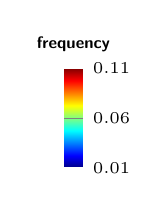
\begin{tikzpicture}
\begin{axis}[font=\bf\sffamily\fontsize{6}{6}\selectfont,
  hide axis,major tick length=0pt,
  xtick=\empty,
    scale only axis,
    height=0pt,
    width=0pt,
    colormap/jet,
    colorbar,
    point meta min=0.01,
    point meta max=0.11,
    colorbar style={title={frequency},title style={yshift=-.05in},font=\bf\sffamily\fontsize{6}{6}\selectfont,draw=none,axis line style={white}, y tick label style={
        /pgf/number format/.cd,
            fixed,
            fixed zerofill,
            precision=2,
        /tikz/.cd
    },  height=.5in,width=.1in,
        ytick={0.01,0.06,0.11}
    }]
    \addplot [draw=none] coordinates {(0,0)};
\end{axis}
\end{tikzpicture}};
  % \node[anchor=north west,label={[]90:{\large b.} 2018-2019 (Northern Hemisphere)}] (T2) at ([xshift=.1in]T1.south west) {
  %   \begin{tikzpicture}[font=\bf\sffamily\fontsize{7}{7}\selectfont]
  %     \node[] (A) at (0,0) {
  %       \mnp{2.65in}{\begin{texshade}{\SEQB}
  %           \shadingmode[chemical]{functional}
  %           \hideallmatchpositions
  %           \rulersteps{1}
  %           \setfont{residues}{sf}{up}{bf}{tiny} 
  %           \setfont{numbering}{sf}{up}{bf}{tiny} 
  %           \setfont{names}{tt}{up}{bf}{small}
  %           \setfont{legend}{tt}{up}{bf}{scriptsize}
  %           \threshold[80]{50}
  %           \setends{1}{1..\LENA}
  %           \showruler{1}{top}
  %           \hideconsensus
  %           \shadeallresidues
  %           \showlegend
  %         \end{texshade}
  %         % 
  %         \begin{texshade}{\SEQB}
  %           %\shadingmode[standard area]{functional}
  %           \shadingmode[hydropathy]{functional}
  %           \hideallmatchpositions
  %           \rulersteps{1}
  %           \setfont{residues}{sf}{up}{bf}{tiny} 
  %           \setfont{numbering}{sf}{up}{bf}{tiny} 
  %           \setfont{names}{tt}{up}{bf}{small}
  %           \setfont{legend}{tt}{up}{bf}{scriptsize}
  %           \threshold[80]{50}
  %           \setends{1}{1..\LENA}
  %           \showruler{1}{top}
  %           \hideconsensus
  %           \shadeallresidues
  %           \showlegend
  %         \end{texshade}
  %         % 
  %         \begin{texshade}{\SEQB}
  %           \shadingmode[accessible area]{functional}
  %           \hideallmatchpositions
  %           \rulersteps{1}
  %           \setfont{residues}{sf}{up}{bf}{tiny}
  %           \setfont{numbering}{sf}{up}{bf}{tiny} 
  %           \setfont{names}{tt}{up}{bf}{small}
  %           \setfont{legend}{tt}{up}{bf}{scriptsize}
  %           \threshold[80]{50}
  %           \setends{1}{1..\LENA}
  %           \showruler{1}{top}
  %           \hideconsensus
  %           \shadeallresidues
  %           \showlegend
  %         \end{texshade}
  %         % 
  %       }};
  %   \end{tikzpicture}};

 %  \node[anchor=north west,label={[]90:{\large c.} 2016-2017 (Southern Hemisphere)}] (T2) at ([xshift=0in]T1.south west) {
%     \begin{tikzpicture}[font=\bf\sffamily\fontsize{7}{7}\selectfont]
%       \node[ ] (A) at (0,0) {
%         \mnp{3.5in}{\begin{texshade}{\SEQC}
%             %\shadingmode[chemical]{functional}
%             \shadingmode[accessible area]{functional}
%             \hideallmatchpositions
%             \rulersteps{1}
%             \setfont{residues}{sf}{up}{bf}{tiny} 
%             \setfont{numbering}{sf}{up}{bf}{tiny} 
%             \setfont{names}{tt}{up}{bf}{small}
%             \setfont{legend}{tt}{up}{bf}{scriptsize}
%             \threshold[80]{50}
%             \setends{1}{1..\LENA}
%             \showruler{1}{top}
%             \hideconsensus
%             \shadeallresidues
%             \showlegend
%           \end{texshade}}};
% \node[] (B) at (A.north east) {  \mnp{3.5in}{      
%           % 
%           \begin{texshade}{\SEQC}
%             %\shadingmode[standard area]{functional}
%             \shadingmode[hydropathy]{functional}
%             \hideallmatchpositions
%             \rulersteps{1}
%             \setfont{residues}{sf}{up}{bf}{tiny} 
%             \setfont{numbering}{sf}{up}{bf}{tiny} 
%             \setfont{names}{tt}{up}{bf}{small}
%             \setfont{legend}{tt}{up}{bf}{scriptsize}
%             \threshold[80]{50}
%             \setends{1}{1..\LENA}
%             \showruler{1}{top}
%             \hideconsensus
%             \shadeallresidues
%             \showlegend
%           \end{texshade}}};


      
%     \end{tikzpicture}};


  

  % \node[anchor=north west,label={[]90:{\large d.} 2016-2017 (Northern Hemisphere)}] (T4) at ([xshift=0in]T3.south west) {
  %   \begin{tikzpicture}[font=\bf\sffamily\fontsize{7}{7}\selectfont]
  %     \node[label={[yshift=-1in,xshift=.15in]170:\mnp{.4in}{\raggedright type \\ \vspace{35pt} sd. chn. area \\ \vspace{35pt} acc. sd. chn.}}] (A) at (0,0) {
  %       \mnp{3.2in}{\begin{texshade}{\SEQD}
  %           \shadingmode[chemical]{functional}
  %           \hideallmatchpositions
  %           \rulersteps{1}
  %           \setfont{residues}{sf}{up}{bf}{tiny} 
  %           \setfont{numbering}{sf}{up}{bf}{tiny} 
  %           \setfont{names}{tt}{up}{bf}{small}
  %           \setfont{legend}{tt}{up}{bf}{scriptsize}
  %           \threshold[80]{50}
  %           \setends{1}{1..\LENA}
  %           \showruler{1}{top}
  %           \hideconsensus
  %           \shadeallresidues
  %           % \showlegend
  %         \end{texshade}
  %         % 
  %         \begin{texshade}{\SEQD}
  %           %\shadingmode[standard area]{functional}
  %           \shadingmode[hydropathy]{functional}
  %           \hideallmatchpositions
  %           \rulersteps{1}
  %           \setfont{residues}{sf}{up}{bf}{tiny} 
  %           \setfont{numbering}{sf}{up}{bf}{tiny} 
  %           \setfont{names}{tt}{up}{bf}{small}
  %           \setfont{legend}{tt}{up}{bf}{scriptsize}
  %           \threshold[80]{50}
  %           \setends{1}{1..\LENA}
  %           \showruler{1}{top}
  %           \hideconsensus
  %           \shadeallresidues
  %           % \showlegend
  %         \end{texshade}
  %         % 
  %         \begin{texshade}{\SEQD}
  %           \shadingmode[accessible area]{functional}
  %           \hideallmatchpositions
  %           \rulersteps{1}
  %           \setfont{residues}{sf}{up}{bf}{tiny}
  %           \setfont{numbering}{sf}{up}{bf}{tiny} 
  %           \setfont{names}{tt}{up}{bf}{small}
  %           \setfont{legend}{tt}{up}{bf}{scriptsize}
  %           \threshold[80]{50}
  %           \setends{1}{1..\LENA}
  %           \showruler{1}{top}
  %           \hideconsensus
  %           \shadeallresidues
  %           % \showlegend
  %         \end{texshade}
  %         % 
  %       }};
  %   \end{tikzpicture}};



  % \node[anchor=north west,label={[]90:{\large e.} 2016-2017 (H3N2 Northern Hemisphere)}] (T5) at ([xshift=0in]T4.south west) {
  %   \begin{tikzpicture}[font=\bf\sffamily\fontsize{7}{7}\selectfont]
  %     \node[label={[yshift=-1in,xshift=.15in]170:\mnp{.4in}{\raggedright type \\ \vspace{35pt} sd. chn. area \\ \vspace{35pt} acc. sd. chn.}}] (A) at (0,0) {
  %       \mnp{3.2in}{\begin{texshade}{\SEQE}
  %           \shadingmode[chemical]{functional}
  %           \hideallmatchpositions
  %           \rulersteps{1}
  %           \setfont{residues}{sf}{up}{bf}{tiny} 
  %           \setfont{numbering}{sf}{up}{bf}{tiny} 
  %           \setfont{names}{tt}{up}{bf}{small}
  %           \setfont{legend}{tt}{up}{bf}{scriptsize}
  %           \threshold[80]{50}
  %           \setends{1}{1..\LENA}
  %           \showruler{1}{top}
  %           \hideconsensus
  %           \shadeallresidues
  %           % \showlegend
  %         \end{texshade}
  %         % 
  %         \begin{texshade}{\SEQE}
  %           %\shadingmode[standard area]{functional}
  %           \shadingmode[hydropathy]{functional}
  %           \hideallmatchpositions
  %           \rulersteps{1}
  %           \setfont{residues}{sf}{up}{bf}{tiny} 
  %           \setfont{numbering}{sf}{up}{bf}{tiny} 
  %           \setfont{names}{tt}{up}{bf}{small}
  %           \setfont{legend}{tt}{up}{bf}{scriptsize}
  %           \threshold[80]{50}
  %           \setends{1}{1..\LENA}
  %           \showruler{1}{top}
  %           \hideconsensus
  %           \shadeallresidues
  %           % \showlegend
  %         \end{texshade}
  %         % 
  %         \begin{texshade}{\SEQE}
  %           \shadingmode[accessible area]{functional}
  %           \hideallmatchpositions
  %           \rulersteps{1}
  %           \setfont{residues}{sf}{up}{bf}{tiny}
  %           \setfont{numbering}{sf}{up}{bf}{tiny} 
  %           \setfont{names}{tt}{up}{bf}{small}
  %           \setfont{legend}{tt}{up}{bf}{scriptsize}
  %           \threshold[80]{50}
  %           \setends{1}{1..\LENA}
  %           \showruler{1}{top}
  %           \hideconsensus
  %           \shadeallresidues
  %           % \showlegend
  %         \end{texshade}
  %         % 
  %       }};
  %   \end{tikzpicture}};


  
\end{tikzpicture}  
  \vspace{0pt}   
  
  \else
  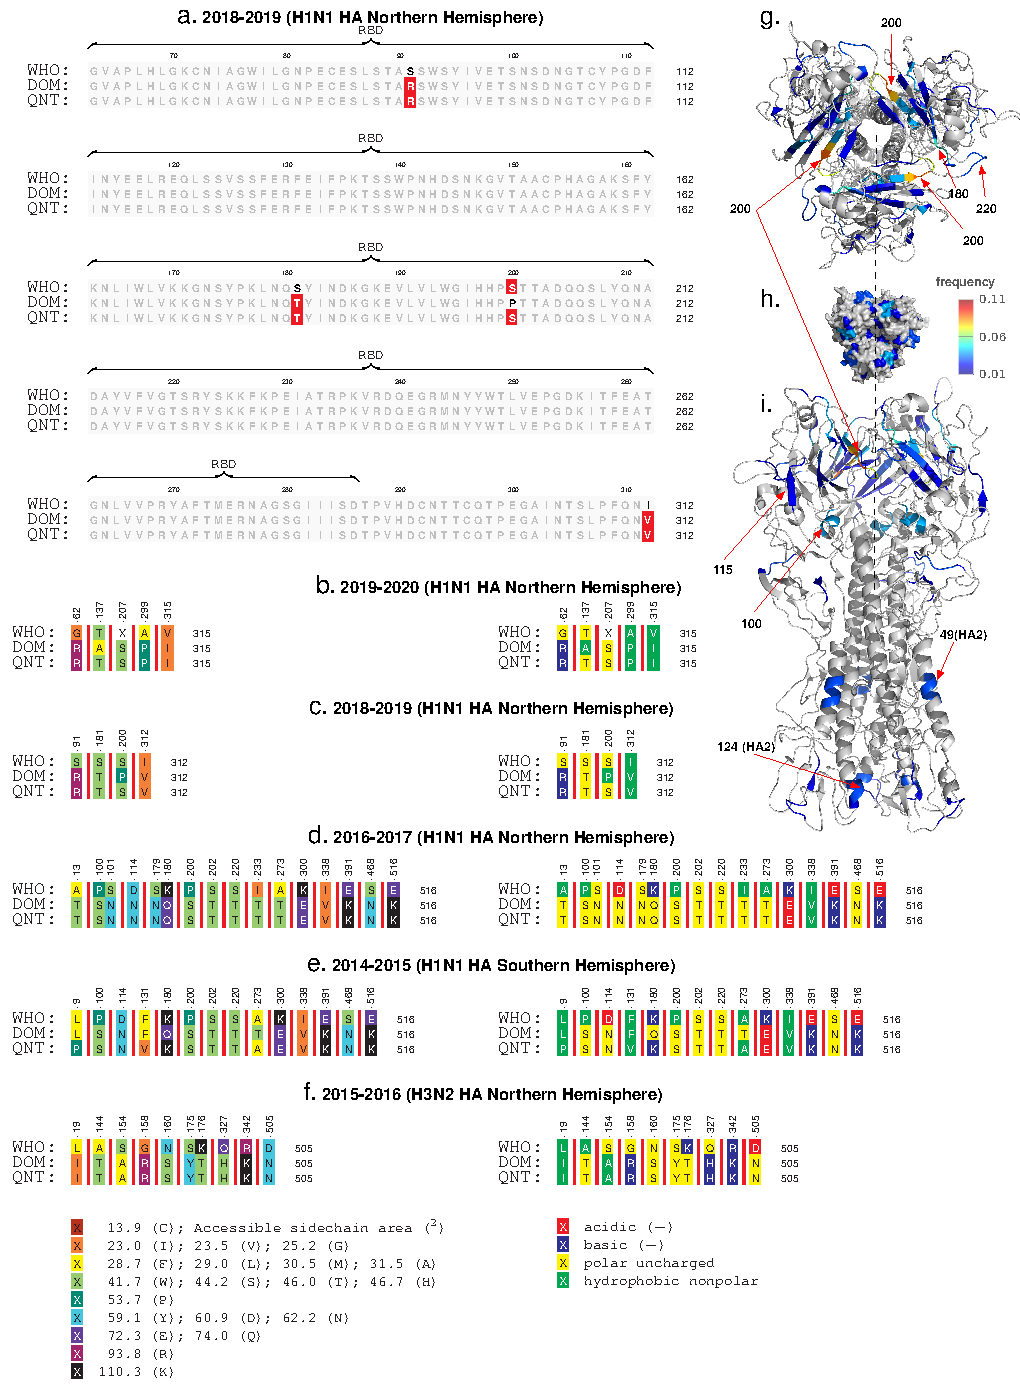
\includegraphics[width=0.87\textwidth]{Figures/External/sequence.pdf}  \vspace{-5pt}   

  \fi
\vspace{0pt}

\captionN{\textbf{Sequence comparisons.} The observed dominant strain, we note that the correct \qnet  deviations tend to be within the RBD, both for H1N1 and H3N2 for HA (panel a shows one example). Additionally, by comparing the type, side chain area, and the accessible side chain area, we note that the changes often have very different properties (panel b-f). Panels g-i show the localization of the deviations in the molecular structure of HA, where we note that the changes are most frequent in the HA1 sub-unit (the globular head), and around residues and structures that have been commonly implicated in receptor binding interactions $e.g$ the $\approx 200$ loop, the $\approx 220$ loop and the $\approx 180$-helix.}\label{figseq}
\end{figure*}
\else
\refstepcounter{figure}\label{figseq}
\fi
%#############################################
%#############################################


%#############################################
%#############################################

\begin{table}\centering
\captionN{Riskiest Strains Currently Circulating in Swine}\label{tabrec11}

\sffamily\fontsize{7}{8}\selectfont

\begin{tabular}{L{2.1in}|L{0.7in}|L{0.7in}|L{0.7in}}\hline
 \rowcolor{lightgray}H1N1 Strain & HA Risk & NA Risk & Overall Risk \\\hline
 A/swine/Tennessee/A02524414/2022 &0.0201&0.0030&0.0077\\\hline
 A/swine/Missouri/A02750646/2022 &0.0201&0.0070&0.0118\\\hline
 A/swine/Kansas/A02711847/2022 &0.0201&0.0098&0.0141\\\hline
 A/swine/Iowa/A02636572/2022 &0.0166&0.0225&0.0193\\\hline
 A/swine/Iowa/A02636308/2021 &0.0143&0.0266&0.0195\\\hline
 A/swine/Illinois/A02750711/2022 &0.0166&0.0233&0.0197\\\hline
 A/swine/Iowa/A02636616/2022 &0.0166&0.0233&0.0197\\\hline
 A/swine/Oklahoma/A02246915/2022 &0.0166&0.0233&0.0197\\\hline
 A/swine/Colorado/A02636469/2022 &0.0166&0.0233&0.0197\\\hline
 A/swine/Iowa/A02636297/2021 &0.0149&0.0267&0.0200\\\hline
 \rowcolor{lightgray}H3N2 Strain & HA Risk & NA Risk & Overall Risk \\\hline
 A/swine/Indiana/A02636492/2022 &0.0104&0.0113&0.0108\\\hline
 A/swine/Indiana/A02636512/2022 &0.0104&0.0113&0.0108\\\hline
 A/swine/Iowa/A02750695/2022 &0.0110&0.0120&0.0115\\\hline
 A/swine/Oklahoma/A02711859/2022 &0.0122&0.0114&0.0118\\\hline
 A/swine/Iowa/A02636351/2022 &0.0121&0.0119&0.0120\\\hline
 A/swine/Iowa/A02636476/2022 &0.0121&0.0120&0.0121\\\hline
 A/swine/Texas/A02636569/2022 &0.0122&0.0120&0.0121\\\hline
 A/swine/Iowa/A02750726/2022 &0.0123&0.0120&0.0121\\\hline
 A/swine/Iowa/A02750740/2022 &0.0104&0.0156&0.0127\\\hline
 A/swine/Indiana/A02636521/2022 &0.0104&0.0156&0.0127\\\hline
 \end{tabular}
\flushleft

\fontsize{7}{7}\selectfont
$^\star$ Converted IRAT Score computed using regression generated from the IRAT vs. Qnet comparison
\end{table}
%#############################################
%#############################################






\clearpage



\section*{Supplementary Figures \& Tables}

\setcounter{figure}{0}
\renewcommand{\figurename}{S-Fig.}
\setcounter{table}{0}
\renewcommand{\tablename}{S-Tab.}
%\setcounter{table}{0}
%\renewcommand{\tablename}{SI Tab.}







%#############################################
%#############################################
\ifFIGS
\begin{figure*}[!ht]
  \centering    
  \tikzexternalenable  
  \tikzsetnextfilename{blastvalid}
  %\tikzXtrue
  \iftikzX 
  \input{Figures/sonet}   
  \vspace{-5pt}    
  
  \else 
  \includegraphics[width=0.9\textwidth]{Figures/External/blastvalid.pdf}
  \fi

  \captionN{\textbf{\qdist validation in-silico using Influenza A sequences from NCBI database. Panel a} illustrates that the \enet induced modeling of evolutionary trajectories initiated from known haemagglutinnin (HA)  sequences  are distinct from random paths in the strain space. In particular, random trajectories have more variance, and more importantly, diverge to different regions of the landscape compared to \enet predictions. \textbf{Panels b-e} show that unconstrained Q-sampling  produces sequences maintain a higher degree of similarity to known sequences, as verified by blasting against known HA sequences, have a smaller rate of growth of variance, and produce matches in closer time frames to the initial sequence. \textbf{Panel c} shows that this is not due to simply restricting the  mutational variations, which increases rapidly in both the \enet and the classical metric.}\label{figsoa}
\end{figure*}
\else
\refstepcounter{figure}\label{figsoa}
\fi
%#############################################
%#############################################


%#############################################
%#############################################
\begin{table*}[!ht]
\def\ACOL{teal!30}
\def\BCOL{Red1!30}
\def\CCOL{gray!30}
\captionN{Examples: \enet induced distance varying for fixed sequence pair when background population changes (rows 1 -5), sequences with small edit distance and large q-distance, and the converse (rows 6-9)}\label{tabex}
\begin{tabular}{L{.1in}|L{.45in}|L{1.85in}|L{2in}|L{.5in}|L{.325in}|L{.325in}}\hline
& Edit dist. & Sequence A & Sequence B & \enet E-dist. & Year A$^\star$ & Year B$^\star$\\\hline
\rowcolor{\ACOL}1&18 & A/Singapore/23J/2007 & A/Tennessee/UR06-0294/2007 & 0.0111 & 2007 & 2007\\\hline
\rowcolor{\ACOL}2&18 & A/Singapore/23J/2007 & A/Tennessee/UR06-0294/2007 & 0.0094 & 2008 & 2008\\\hline
\rowcolor{\ACOL}3&18 & A/Singapore/23J/2007 & A/Tennessee/UR06-0294/2007 & 0.0027 & 2009 & 2009\\\hline
\rowcolor{\ACOL}4&18 & A/Singapore/23J/2007 & A/Tennessee/UR06-0294/2007 & 0.0025 & 2010 & 2010\\\hline
\rowcolor{\ACOL}5&18 & A/Singapore/23J/2007 & A/Tennessee/UR06-0294/2007 & 0.6163 & 2007 & 2010\\\hline
\rowcolor{\BCOL}6&11 & A/Naypyitaw/M783/2008 & A/Singapore/201/2008 &      0.8852 & 2008 & 2008\\\hline
\rowcolor{\BCOL}7&15 & A/Cambodia/W0908339/2012 & A/Singapore/DMS1233/2012&0.2737 & 2012 & 2012\\\hline
\rowcolor{\CCOL}8&126 & A/South Dakota/03/2008 & A/Singapore/10/2008 &     0.3034 & 2008 & 2008\\\hline
\rowcolor{\CCOL}9&141 & A/Jodhpur/3248/2012 & A/Cambodia/W0908339/2012 &   0.2405 & 2012 & 2012\\\hline
\end{tabular}
\flushleft
$^\star$Year A and year B correspond to the assumed collection years for sequences A and B respectively for the purpose of this example. Sequence A in row 1 is collected in 2007, but is assumed to be from different years in rows 2-4 to demonstrate the change in q-distance from sequence B, arising only from a change in the background population.
\end{table*}
%#############################################
%#############################################




%#############################################
%#############################################
\begin{table*}[!ht]
 \mnp{2.75in}{ \centering
 \captionN{Correlation between \qdist and edit distance between sequence pairs}\label{tabcor}
\sffamily\fontsize{8}{8}\selectfont
\begin{tabular}{L{1.35in}|L{.65in}}\hline
Phenotypes & Correlation \\\hline
 Influenza H1N1 HA  &0.76\\\hline
 Influenza H1N1 NA &0.74\\\hline
 Influenza H3N2 HA &0.85\\\hline
 Influenza H3N2 NA &0.79\\\hline
% \hcov &0.52\\\hline
\end{tabular}
}\hfill
\mnp{3.75in}{  \centering
 \captionN{Number of sequences collected from public databases}\label{tabseq}
\sffamily\fontsize{8}{8}\selectfont
\begin{tabular}{L{.7in}|L{1.55in}|L{.95in}}\hline
Database & Strain & No. of Sequences \\\hline
NCBI& Influenza  H1N1  HA &17,894\\\hline
NCBI& Influenza  H1N1  NA &16,637\\\hline
NCBI& Influenza  H3N2  HA &18,265\\\hline
NCBI& Influenza  H3N2  NA &14,699\\\hline
GISAID& Influenza  H1N1  HA &1,528\\\hline
GISAID& Influenza  H1N1  NA &1,490\\\hline
GISAID& Influenza  H3N2  HA &13,975\\\hline
GISAID& Influenza  H3N2  NA &13,811\\\hline
Total & &98,299\\\hline
\end{tabular}
}
\end{table*}
%#############################################
%#############################################


%#############################################
%#############################################
\ifFIGS
\begin{figure*}[!ht]
  \centering
  \tikzexternalenable
  \tikzsetnextfilename{dom}

  \iftikzX
  
\begin{tikzpicture}[font=\bf\sffamily\fontsize{8}{8}\selectfont]
\def\DATAA{Figures/plotdata/h1n1humanHA_dom_ldist.dat}
\def\DATAB{Figures/plotdata/h1n1humanNA_dom_ldist.dat}
\def\DATAC{Figures/plotdata/h3n2humanHA_dom_ldist.dat}
\def\DATAD{Figures/plotdata/h3n2humanNA_dom_ldist.dat}

\node[] (A) at (0,0) {
\begin{tikzpicture}
\begin{groupplot}[group style={
        group size=2 by 2,
        xlabels at=edge bottom,
        xticklabels at=edge bottom,
        vertical sep=0.2in, horizontal sep=.35in,
    },height=2in,width=2in]

\nextgroupplot[ylabel=probability,ylabel style={xshift=-.8in,yshift=-.1in}]
\addplot [
    hist={
        bins=50,
        data min=0,
        data max=30,
density=true
    }  , fill=black!50
] table [y index=0] {\DATAA};
\addlegendentry{HA H1N1}


\nextgroupplot[]
\addplot [
    hist={
        bins=50,
        data min=0,
        data max=30,
density=true
    }    , fill=black!50
] table [y index=0] {\DATAB};
\addlegendentry{NA H1N1}


\nextgroupplot[xlabel=Edit Distance from Dominant Strain,xlabel style={xshift=.8in}]
\addplot [
    hist={
        bins=50,
        data min=0,
        data max=30,
density=true
    }    , fill=black!50
] table [y index=0] {\DATAC};
\addlegendentry{HA H3N2}


\nextgroupplot[]
\addplot [
    hist={
        bins=50,
        data min=0,
        data max=30,
density=true
    }    , fill=black!50
] table [y index=0] {\DATAD};
\addlegendentry{NA H3N2}


\end{groupplot}
\end{tikzpicture}
};

\node [anchor=south west] (L1) at (A.north west) {{\large a.} Distribution around dominant strain};

\end{tikzpicture}

  
  \else
  \includegraphics[width=.6\textwidth]{Figures/External/dom.pdf}
  \vspace{0pt}
  \fi
  
\vspace{0pt}

\captionN{\textbf{No. of mutations from the seasonal dominant strain over the years} The quasispecies that circulates each season for each sub-type is tightly distributed around the dominant strain on average.}\label{figdom}
\end{figure*}
\else
\refstepcounter{figure}\label{figdom}
\fi
%#############################################
%#############################################





% \begin{table}[!ht]\centering
% \captionN{H1N1 NA Northern Hemisphere}\label{tabrec2}

% \sffamily\fontsize{7}{8}\selectfont

% \begin{tabular}{L{.37in}|L{1.62in}|L{1.62in}|L{1.62in}|L{.25in}|L{.25in}}\hline
Year & WHO Recommendation & Dominant Strain & \qnet Recommendation & WHO Error & \qnet Error \\\hline
2001-02& A/New  Caledonia/20/99 & A/New  York/447/2001 & A/Memphis/15/2000 &4&4\\\hline
2002-03& A/New  Caledonia/20/99 & A/Paris/0833/2002 & A/New  York/341/2001 &1&5\\\hline
2003-04& A/New  Caledonia/20/99 & A/Memphis/5/2003 & A/New  York/291/2002 &3&5\\\hline
2004-05& A/New  Caledonia/20/99 & A/Singapore/14/2004 & A/New  York/223/2003 &2&3\\\hline
2005-06& A/New  Caledonia/20/99 & A/Taiwan/5524/2005 & A/Florida/3e/2004 &3&0\\\hline
2006-07& A/New  Caledonia/20/99 & A/Massachusetts/08/2006 & A/Sofia/361/2005 &4&2\\\hline
2007-08& A/Solomon  Islands/3/2006 & A/Tennessee/UR06-0106/2007 & A/Sofia/490/2006 &9&2\\\hline
2008-09& A/Brisbane/59/2007 & A/Sendai/TU66/2008 & A/Maryland/04/2007 &0&3\\\hline
2009-10& A/Brisbane/59/2007 & A/Thailand/SR08021/2009 & A/Paris/910/2008 &87&87\\\hline
2010-11& A/California/7/2009 & A/Finland/2460N/2010 & A/Rome/709/2009 &2&9\\\hline
2011-12& A/California/7/2009 & A/Tula/CRIE-GSYu/2011 & A/Oman/SQUH-40/2010 &4&2\\\hline
2012-13& A/California/7/2009 & A/Bangalore/697-32/2012 & A/Nizhnii  Novgorod/CRIE-ZCA/2011 &4&0\\\hline
2013-14& A/California/7/2009 & A/Jiangsugusu/SWL1824/2013 & A/LongYan/SWL33/2013 &5&3\\\hline
2014-15& A/California/7/2009 & A/LongYan/SWL2457/2014 & A/Utah/06/2013 &9&3\\\hline
2015-16& A/California/7/2009 & A/Michigan/45/2015 & A/Maryland/02/2014 &14&4\\\hline
2016-17& A/California/7/2009 & A/Mexico/4436/2016 & A/India/Pun151245/2015 &14&0\\\hline
2017-18& A/Michigan/45/2015 & A/Illinois/37/2017 & A/Utah/02/2016 &3&3\\\hline
2018-19& A/Michigan/45/2015 & A/Kenya/47/2018 & A/Maine/24/2017 &4&0\\\hline
2019-20& A/Brisbane/02/2018 & A/Texas/7939/2019 & A/Missouri/03/2018 &1&0\\\hline
2020-21& A/Hawaii/70/2019 &A/Togo/897/2020& A/Texas/112/2019 &0&5\\\hline
2021-22& A/Victoria/2570/2019 &A/Cote\_d'Ivoire/3729/2021&A/Togo/0071/2021&1&5\\\hline
2022-23& -1 &-1& A/Lyon/820/2021 &-1&-1\\\hline
\end{tabular}

% \flushleft

% \fontsize{7}{7}\selectfont
% $^\star$ Dominant strain is calculated as the one closest to the centroid in the strain space that year in the edit distance metric
% \end{table}
% %#############################################
% %#############################################

% \begin{table}[!ht]\centering
% \captionN{H1N1 NA Southern Hemisphere}\label{tabrec3}

% \sffamily\fontsize{7}{8}\selectfont

% \begin{tabular}{L{.37in}|L{1.62in}|L{1.62in}|L{1.62in}|L{.25in}|L{.25in}}\hline
Year & WHO Recommendation & Dominant Strain & \qnet Recommendation & WHO Error & \qnet Error \\\hline
2001-02& A/New  Caledonia/20/99 & A/New  York/447/2001 & A/Canterbury/37/2000 &4&6\\\hline
2002-03& A/New  Caledonia/20/99 & A/Paris/0833/2002 & A/New  York/447/2001 &1&5\\\hline
2003-04& A/New  Caledonia/20/99 & A/Memphis/5/2003 & A/New  York/291/2002 &3&5\\\hline
2004-05& A/New  Caledonia/20/99 & A/Singapore/14/2004 & A/Memphis/5/2003 &2&3\\\hline
2005-06& A/New  Caledonia/20/99 & A/Taiwan/5524/2005 & A/Canterbury/106/2004 &3&6\\\hline
2006-07& A/New  Caledonia/20/99 & A/Massachusetts/08/2006 & A/Sofia/361/2005 &4&2\\\hline
2007-08& A/New  Caledonia/20/99 & A/Tennessee/UR06-0106/2007 & A/Thailand/RMSC-UDN-20/2006 &4&8\\\hline
2008-09& A/Solomon  Islands/3/2006 & A/Sendai/TU66/2008 & A/Tennessee/UR06-0151/2007 &15&13\\\hline
2009-10& A/Brisbane/59/2007 & A/Thailand/SR08021/2009 & A/Nebraska/07/2008 &87&87\\\hline
2010-11& A/California/7/2009 & A/Finland/2460N/2010 & A/Rome/709/2009 &2&9\\\hline
2011-12& A/California/7/2009 & A/Tula/CRIE-GSYu/2011 & A/Finland/2460N/2010 &4&2\\\hline
2012-13& A/California/7/2009 & A/Bangalore/697-32/2012 & A/Tula/CRIE-GSYu/2011 &4&0\\\hline
2013-14& A/California/7/2009 & A/Jiangsugusu/SWL1824/2013 & A/Oman/SQUH-63/2012 &5&4\\\hline
2014-15& A/California/7/2009 & A/LongYan/SWL2457/2014 & A/NanPing/SWL1640/2013 &9&6\\\hline
2015-16& A/California/7/2009 & A/Michigan/45/2015 & A/LongYan/SWL2457/2014 &14&5\\\hline
2016-17& A/California/7/2009 & A/Mexico/4436/2016 & A/Michigan/45/2015 &14&0\\\hline
2017-18& A/Michigan/45/2015 & A/Illinois/37/2017 & A/Mexico/4436/2016 &3&3\\\hline
2018-19& A/Michigan/45/2015 & A/Kenya/47/2018 & A/Kentucky/26/2017 &4&2\\\hline
2019-20& A/Michigan/45/2015 & A/Texas/7939/2019 & A/Kenya/47/2018 &4&0\\\hline
2020-21& A/Brisbane/02/2018 &A/Togo/897/2020& A/Texas/7939/2019 &6&5\\\hline
2021-22& A/Victoria/2570/2019 &A/Cote\_D'Ivoire/1496/2021& A/NAGASAKI/8/2020 &1&6\\\hline
2022-23& -1 &-1& A/Dakar/35/2021 &-1&-1\\\hline
\end{tabular}

% \flushleft

% \fontsize{7}{7}\selectfont
% $^\star$ Dominant strain is calculated as the one closest to the centroid in the strain space that year in the edit distance metric
% \end{table}


% \begin{table}[!ht]\centering
% \captionN{H3N2 NA Northern Hemisphere}\label{tabrec6}

% \sffamily\fontsize{7}{8}\selectfont

% \begin{tabular}{L{.37in}|L{1.62in}|L{1.62in}|L{1.62in}|L{.25in}|L{.25in}}\hline
Year & WHO Recommendation & Dominant Strain & \qnet Recommendation & WHO Error & \qnet Error \\\hline
2003-04&A/Moscow/10/99& A/Denmark/107/2003 & A/New  York/100/2002 &13&3\\\hline
2004-05& A/Fujian/411/2002 &A/Hyogo/36/2004& A/New  York/20/2003 &3&16\\\hline
2005-06& A/California/7/2004 & A/Denmark/203/2005 & A/Hong  Kong/HKU20/2004 &4&0\\\hline
2006-07& A/Wisconsin/67/2005 & A/Berlin/32/2006 & A/Mexico/InDRE2227/2005 &1&1\\\hline
2007-08& A/Wisconsin/67/2005 & A/Brazil/80/2007 & A/Baden-Wuerttemberg/17/2006 &8&7\\\hline
2008-09& A/Brisbane/10/2007 & A/Missouri/05/2008 & A/Washington/01/2007 &3&2\\\hline
2009-10& A/Brisbane/10/2007 & A/Oklahoma/09/2009 & A/Wisconsin/24/2008 &3&1\\\hline
2010-11& A/Perth/16/2009 & A/California/17/2010 & A/New  York/70/2009 &2&3\\\hline
2011-12& A/Perth/16/2009 & A/Texas/14/2011 & A/California/14/2010 &3&2\\\hline
2012-13& A/Victoria/361/2011 & A/New  York/02/2012 & A/Singapore/C2011.493/2011 &4&1\\\hline
2013-14& A/Victoria/361/2011 & A/Michigan/02/2013 & A/New  York/01/2012 &3&1\\\hline
2014-15& A/Texas/50/2012 & A/Tehran/69634/2014 & A/Boston/DOA2-176/2013 &3&1\\\hline
2015-16& A/Switzerland/9715293/2013 &A/Parma/471/2015& A/Thailand/CU-B10520/2014 &3&0\\\hline
2016-17& A/Hong  Kong/4801/2014 & A/North  Carolina/62/2016 & A/Delaware/02/2015 &7&2\\\hline
2017-18& A/Hong  Kong/4801/2014 & A/Texas/277/2017 & A/New  York/03/2016 &8&0\\\hline
2018-19& A/Singapore/INFIMH-16-0019/2016 & A/Japan/NHRC\_FDX70352/2018 & A/Colorado/11/2017 &4&3\\\hline
2019-20& A/Kansas/14/2017 & A/Washington/9757/2019 &A/Guangxi-Fangcheng/54/2019&3&11\\\hline
2020-21& A/Hong  Kong/2671/2019 & A/Bangladesh/1004005/2020 & A/Maryland/02/2019 &3&13\\\hline
2021-22& A/Cambodia/e0826360/2020 &A/Stockholm/10/2022& A/Bangladesh/1916/2020 &2&2\\\hline
2022-23& -1 &-1& A/Iowa/20/2022 &-1&-1\\\hline
\end{tabular}

% \flushleft

% \fontsize{8}{8}\selectfont
% $^\star$ Dominant strain is calculated as the one closest to the centroid in the strain space that year in the edit distance metric
% \end{table}
% \vspace{100pt}
% %#############################################
% %#############################################

% \begin{table}[!ht]\centering
% \captionN{H3N2 NA Southern Hemisphere}\label{tabrec7}

% \sffamily\fontsize{7}{8}\selectfont

% \begin{tabular}{L{.37in}|L{1.62in}|L{1.62in}|L{1.62in}|L{.25in}|L{.25in}}\hline
Year & WHO Recommendation & Dominant Strain & \qnet Recommendation & WHO Error & \qnet Error \\\hline
2003-04&A/Moscow/10/99& A/Denmark/107/2003 & A/New  York/101/2002 &13&3\\\hline
2004-05& A/Fujian/411/2002 &A/Hyogo/36/2004& A/New  York/20/2003 &3&16\\\hline
2005-06& A/Wellington/1/2004 & A/Denmark/203/2005 & A/Wellington/1/2004 &2&2\\\hline
2006-07& A/California/7/2004 & A/Berlin/32/2006 & A/Mexico/InDRE2227/2005 &3&1\\\hline
2007-08& A/Wisconsin/67/2005 & A/Brazil/80/2007 & A/Ohio/06/2006 &8&10\\\hline
2008-09& A/Brisbane/10/2007 & A/Missouri/05/2008 & A/Brazil/80/2007 &3&2\\\hline
2009-10& A/Brisbane/10/2007 & A/Oklahoma/09/2009 & A/Wisconsin/24/2008 &3&1\\\hline
2010-11& A/Perth/16/2009 & A/California/17/2010 & A/New  York/70/2009 &2&3\\\hline
2011-12& A/Perth/16/2009 & A/Texas/14/2011 & A/Virginia/05/2010 &3&2\\\hline
2012-13& A/Perth/16/2009 & A/New  York/02/2012 & A/Texas/14/2011 &4&1\\\hline
2013-14& A/Victoria/361/2011 & A/Michigan/02/2013 & A/New  York/02/2012 &3&3\\\hline
2014-15& A/Texas/50/2012 & A/Tehran/69634/2014 & A/Michigan/02/2013 &3&1\\\hline
2015-16& A/Switzerland/9715293/2013 &A/Parma/471/2015& A/Tehran/69634/2014 &3&2\\\hline
2016-17& A/Hong  Kong/4801/2014 & A/North  Carolina/62/2016 &A/Parma/471/2015&7&2\\\hline
2017-18& A/Hong  Kong/4801/2014 & A/Texas/277/2017 & A/Guangdong/264/2016 &8&0\\\hline
2018-19& A/Singapore/INFIMH-16-0019/2016 & A/Japan/NHRC\_FDX70352/2018 & A/Texas/277/2017 &4&3\\\hline
2019-20& A/Switzerland/8060/2017 & A/Washington/9757/2019 & A/Pennsylvania/317/2018 &10&10\\\hline
2020-21& A/South  Australia/34/2019 & A/Bangladesh/1004005/2020 & A/Washington/9757/2019 &1&13\\\hline
2021-22& A/Hong Kong/2671/2019 &A/India/PUN-NIV301718/2021	& A/Darwin/11/2021 &6&1\\\hline
2022-23& -1 &-1& A/Texas/12723/2022 &-1&-1\\\hline
\end{tabular}

% \flushleft

% \fontsize{7}{7}\selectfont
% $^\star$ Dominant strain is calculated as the one closest to the centroid in the strain space that year in the edit distance metric
% \end{table}
% %#############################################
% %#############################################





%#############################################
%#############################################

\begin{table}\centering
\captionN{H1N1 NA Northern Hemisphere (Multi-cluster)}\label{tabrec8}

\sffamily\fontsize{7}{8}\selectfont

\input{Figures/tabdata/north_h1n1_na_3cluster.tex}
\flushleft

\fontsize{7}{7}\selectfont
$^\star$ Dominant strain is calculated as the one closest to the centroid in the strain space that year in the edit distance metric
\end{table}

%#############################################
%#############################################

\begin{table}\centering
\captionN{H1N1 NA Southern Hemisphere (Multi-cluster)}\label{tabrec9}

\sffamily\fontsize{7}{8}\selectfont

\begin{tabular}{L{.37in}|L{1.33in}|L{.25in}|L{.25in}|L{.25in}|L{1.65in}|L{1.65in}}\hline
Year & WHO Recommendation & WHO Error & \qnet Error 1 & \qnet Error 2 & \qnet Recommendation 1 & \qnet  Recommendation 2 \\\hline
2001-02& A/New  Caledonia/20/99 &4&1&6& A/New  South  Wales/26/2000 & A/Canterbury/37/2000 \\\hline
2002-03& A/New  Caledonia/20/99 &1&0&5& A/Wellington/1/2001 & A/New  York/447/2001 \\\hline
2003-04& A/New  Caledonia/20/99 &3&2&8& A/Paris/0833/2002 & A/Taiwan/141/2002 \\\hline
2004-05& A/New  Caledonia/20/99 &2&3&4& A/Memphis/5/2003 & A/Hanoi/1004/2003 \\\hline
2005-06& A/New  Caledonia/20/99 &3&0&1& A/Denmark/130/2004 & A/Paris/650/2004 \\\hline
2006-07& A/New  Caledonia/20/99 &4&2&8& A/Sofia/361/2005 & A/Wellington/11/2005 \\\hline
2007-08& A/New  Caledonia/20/99 &4&4&8& A/Sofia/246/2006 & A/New  York/8/2006 \\\hline
2008-09& A/Solomon  Islands/3/2006 &15&13&19& A/Tennessee/UR06-0151/2007 & A/Ohio/UR06-0178/2007 \\\hline
2009-10& A/Brisbane/59/2007 &87&88&90& A/Sendai/TU66/2008 & A/Japan/618/2008 \\\hline
2010-11& A/California/7/2009 &2&1&6& A/South  Carolina/WRAIR1645P/2009 & A/Wisconsin/629-D00809/2009 \\\hline
2011-12& A/California/7/2009 &4&1&3& A/England/21680633/2010 & A/Hangzhou/178/2010 \\\hline
2012-13& A/California/7/2009 &4&1&22& A/Joshkar-Ola/CRIE-BLP/2011 & A/Rio Grande do Sul/578/2011 \\\hline
2013-14& A/California/7/2009 &5&4&13& A/Thailand/MR10580/2012 & A/Mexico/INMEGEN-INER  15/2012 \\\hline
2014-15& A/California/7/2009 &9&3&7& A/Minnesota/02/2013 & A/Helsinki/430/2013 \\\hline
2015-16& A/California/7/2009 &14&4&7& A/Helsinki/808M/2014 & A/Virginia/NHRC430739/2014 \\\hline
2016-17& A/California/7/2009 &14&0&3& A/Michigan/45/2015 & A/Colorado/30/2015 \\\hline
2017-18& A/Michigan/45/2015 &3&3&8& A/Mexico/4436/2016 & A/Arizona/03/2016 \\\hline
2018-19& A/Michigan/45/2015 &4&0&4& A/California/NHRC\_QV11073/2017 & A/Minnesota/35/2017 \\\hline
2019-20& A/Michigan/45/2015 &4&0&2& A/Kenya/47/2018 & A/Colorado/7682/2018 \\\hline
2020-21& A/Brisbane/02/2018 &5&2&7& A/California/NHRC-OID\_BOX-ILI-0012/2019 & A/Indiana/30/2019 \\\hline
2021-22& A/Victoria/2570/2019 &1&7&58& A/Togo/0155/2021 & A/Shandong/00204/2021 \\\hline
2022-23& -1 &-1&-1&-1& A/Switzerland/86136/2022 & A/Wisconsin/04/2021 \\\hline
\end{tabular}
\flushleft

\fontsize{7}{7}\selectfont
$^\star$ Dominant strain is calculated as the one closest to the centroid in the strain space that year in the edit distance metric
\end{table}

%#############################################
%#############################################

\begin{table}\centering
\captionN{H3N2 NA Northern Hemisphere (Multi-cluster)}\label{tabrec10}

\sffamily\fontsize{7}{8}\selectfont

\input{Figures/tabdata/north_h3n2_na_3cluster.tex}
\flushleft

\fontsize{7}{7}\selectfont
$^\star$ Dominant strain is calculated as the one closest to the centroid in the strain space that year in the edit distance metric
\end{table}

%#############################################
%#############################################

\begin{table}\centering
\captionN{H3N2 NA Southern Hemisphere (Multi-cluster)}\label{tabrec11}

\sffamily\fontsize{7}{8}\selectfont

\begin{tabular}{L{.37in}|L{1.33in}|L{.25in}|L{.25in}|L{.25in}|L{1.65in}|L{1.65in}}\hline
Year & WHO Recommendation & WHO Error & \qnet Error 1 & \qnet Error 2 & \qnet Recommendation 1 & \qnet  Recommendation 2 \\\hline
2003-04&A/Moscow/10/99&13&4&5& A/Auckland/612/2002 & A/New  York/87/2002 \\\hline
2004-05& A/Fujian/411/2002 &3&16&18& A/New  York/20/2003 & A/New  York/12/2003 \\\hline
2005-06& A/Wellington/1/2004 &2&1&7& A/New  York/358/2004 & A/Singapore/36/2004 \\\hline
2006-07& A/California/7/2004 &3&3&8&A/Macau/557/2005& A/Hong  Kong/HKU53/2005 \\\hline
2007-08& A/Wisconsin/67/2005 &8&0&10& A/Wisconsin/42/2006 & A/Wisconsin/44/2006 \\\hline
2008-09& A/Brisbane/10/2007 &3&4&10& A/Missouri/06/2007 & A/Japan/72/2007 \\\hline
2009-10& A/Brisbane/10/2007 &3&1&7& A/Wisconsin/24/2008 & A/Mississippi/UR07-0042/2008 \\\hline
2010-11& A/Perth/16/2009 &2&3&8& A/New  York/70/2009 & A/Japan/883/2009 \\\hline
2011-12& A/Perth/16/2009 &3&2&2& A/California/19/2010 & A/Virginia/05/2010 \\\hline
2012-13& A/Perth/16/2009 &4&1&12& A/Texas/14/2011 & A/Singapore/GP1684/2011 \\\hline
2013-14& A/Victoria/361/2011 &3&1&5& A/Idaho/38/2012 & A/Pavia/135/2012 \\\hline
2014-15& A/Texas/50/2012 &3&1&1& A/Nevada/05/2013 & A/Michigan/02/2013 \\\hline
2015-16& A/Switzerland/9715293/2013 &3&0&4& A/Nicaragua/6866\_14/2014 & A/Iran/91244/2014 \\\hline
2016-17& A/Hong Kong/4801/2014 &7&1&25& A/New  Jersey/13/2015 & A/California/NHRC\_BRD41056N/2015 \\\hline
2017-18& A/Hong Kong/4801/2014 &9&1&4& A/Guangdong/264/2016 & A/Victoria/668/2016 \\\hline
2018-19& A/Singapore/INFIMH-16-0019/2016 &3&2&4& A/Netherlands/3530/2017 & A/Washington/17/2017 \\\hline
2019-20& A/Switzerland/8060/2017 &10&4&10& A/England/538/2018 & A/California/BRD12490N/2018 \\\hline
2020-21& A/South  Australia/34/2019 &1&1&13& A/England/9738/2019 & A/Washington/9757/2019 \\\hline
2021-22& A/Hong Kong/2671/2019 &6&1&49& A/Darwin/11/2021 & A/Hawaii/28/2020 \\\hline
2022-23& -1 &-1&-1&-1& A/Congo/313/2021	 & A/Texas/12723/2022 \\\hline
\end{tabular}
\flushleft

\fontsize{7}{7}\selectfont
$^\star$ Dominant strain is calculated as the one closest to the centroid in the strain space that year in the edit distance metric
\end{table}
%#############################################
% %#############################################
% %#############################################
% \ifFIGS
% \begin{figure*}[!t]
%   \centering    
%   %\tikzexternalenable  
%   %\tikzsetnextfilename{IRAT_split.png}
%   %\iftikzX 
%   %\vspace{-5pt}    
  
%   %\else 
%   \includegraphics[width=0.9\textwidth]{Figures/External/IRAT_split.png}
%   %\fi

%   \captionN{\textbf{IRAT vs. Q-distance relationship for H1- and H3- sub-types, using past year data vs. using all data.} On the result when computing average q-distance between the target strain and the circulating human strains from the past year, and on the right is the result when using all available human strains of that sub-type. Evidently, the former has a much higher correlation, since a strain being ``close" to humans at some point does not necessarily mean being close now.}\label{irat}
% \end{figure*}
% \else
% \refstepcounter{figure}\label{irat}
% \fi
% %#############################################
% %#############################################





%#############################################
%#############################################

\begin{table}[!ht]\centering
\captionN{Influenza A Strains Evaluated by IRAT and Corresponding \enet Computed Risk Scores}\label{irattab}

\sffamily\fontsize{7}{8}\selectfont

\begin{tabular}{L{1.32in}|L{.35in}|L{.3in}|L{.3in}|L{.3in}|L{.35in}|L{.35in}|L{.35in}|L{.35in}|L{.32in}|L{.3in}|L{.3in}}\hline
Influenza Virus & Subype & IRAT Date &IRAT Emergence Score &IRAT Impact Score &HA Enet Sample &NA Enet Sample &HA Avg. E-dist. &NA Avg. E-dist. &Geom. Mean&Enet Emergence Score&Enet Impact Score \\\hline
 A/swine/Shandong/1207/2016 &H1N1& Jul  2020 &7.5&6.9&1000&1000&0.0941&0.0205&0.0440&6.00&6.06\\\hline
 A/Ohio/13/2017 &H3N2& Jul  2019 &6.6&5.8&1000&1000&0.0184&0.0306&0.0238&6.34&6.34\\\hline
 A/Hong  Kong/125/2017 &H7N9& May  2017 &6.5&7.5&437&437&0.0296&0.0058&0.0131&6.54&6.49\\\hline
 A/Shanghai/02/2013 &H7N9& Apr  2016 &6.4&7.2&178&178&0.0055&0.0036&0.0044&6.70&6.62\\\hline
 A/Anhui-Lujiang/39/2018 &H9N2& Jul  2019 &6.2&5.9&31&30&0.0290&0.1681&0.0698&5.58&5.74\\\hline
 A/Indiana/08/2011 &H3N2& Dec  2012 &6.0&4.5&1000&1000&0.0523&0.0091&0.0218&6.37&6.36\\\hline
 A/California/62/2018 &H1N2& Jul  2019 &5.8&5.7&55&55&0.1089&0.0610&0.0815&5.41&5.61\\\hline
 A/Bangladesh/0994/2011$^{\star\star\star}$ &H9N2& Feb  2014 &5.6&5.4&-1&-1&0.2078&0.1823&0.1947&4.21&4.69\\\hline
 A/Sichuan/06681/2021 &H5N6& Oct  2021 &5.3&6.3&45&45&0.3616&0.0518&0.1369&4.72&5.07\\\hline
 A/Vietnam/1203/2004 &H5N1& Nov  2011 &5.2&6.6&258&246&0.1673&0.0111&0.0430&6.01&6.07\\\hline
 A/Yunnan/14564/2015$^{\star\star}$ &H5N6& Apr  2016 &5.0&6.6&344&331&0.3482&0.2987&0.3225&3.80&4.45\\\hline
 A/Astrakhan/3212/2020$^{\star\star}$ &H5N8& Mar  2021 &4.6&5.2&381&365&0.1603&0.3472&0.2359&3.97&4.53\\\hline
 A/Netherlands/219/2003 &H7N7& Jun  2012 &4.6&5.8&46&46&0.2757&0.3521&0.3115&3.80&4.45\\\hline
 A/American  wigeon/South  Carolina/AH0195145/2021 &H5N1& Mar  2022 &4.4&5.1&335&323&0.1722&0.5114&0.2967&3.81&4.45\\\hline
 A/Jiangxi-Donghu/346/2013$^{\star\star\star}$ &H10N8& Feb  2014 &4.3&6.0&-1&-1&0.2088&0.2101&0.2094&4.11&4.62\\\hline
 A/gyrfalcon/Washington/ 41088/2014$^{\star\star}$ &H5N8& Mar  2015 &4.2&4.6&341&328&0.1532&0.3424&0.2290&4.00&4.55\\\hline
 A/Northern  pintail/ Washington/40964/2014$^{\star\star}$ &H5N2& Mar  2015 &3.8&4.1&341&328&0.1529&0.3799&0.2410&3.95&4.51\\\hline
 A/canine/Illinois/12191/2015 &H3N2& Jun  2016 &3.7&3.7&1000&1000&0.0607&0.1509&0.0957&5.22&5.45\\\hline
 A/American  green-winged  teal /Washington/1957050/2014 &H5N1& Mar 2015 &3.6&4.1&326&314&0.1911&0.4482&0.2927&3.82&4.45\\\hline
 A/turkey/Indiana/1573-2/2016$^{\star\star}$ &H7N8& Jul  2017 &3.4&3.9&495&494&0.1130&0.7738&0.2957&3.81&4.45\\\hline
 A/chicken/Tennessee/17-007431-3/2017 &H7N9& Oct  2017 &3.1&3.5&496&495&0.1027&0.2569&0.1624&4.47&4.88\\\hline
 A/chicken/Tennessee/17-007147-2/2017 &H7N9& Oct  2017 &2.8&3.5&496&495&0.2095&0.2541&0.2307&3.99&4.54\\\hline
 A/duck/New  York/1996 $^\star$&H1N1& Nov  2011 &2.3&2.4&1000&1000&-1&-1&-1&-1&-1\\\hline
 \end{tabular}
\flushleft

\fontsize{8}{8}\selectfont
$^\star$ HA strain is not available for A/duck/New York/1996, so this strain is omitted.\\
$^{\star\star}$ Could not construct a \enet of human sequence data available for that virus sub-type (less than 30 strains), so we constructed a \enet using all human strains that match the HA sub-type, i.e. H5NX for H5N6.\\
$^{\star\star\star}$ These strains did not have enough human sequence data to generate a \enet, even when only considering the HA sub-type. Thus, we estimated the risk score using every \enet from the other IRAT strains, and took the average among NA and HA. Finally, we took the geometric mean of the resulting NA and HA averages.
\end{table}

%#############################################


%#############################################
\ifFIGS
%#############################################

\begin{table}[!ht]\centering
\captionN{Influenza A Strains Evaluated by IRAT and Corresponding \enet Computed Current Risk Scores}\label{irattab_current}

\sffamily\fontsize{7}{8}\selectfont

\begin{tabular}{L{1.25in}|L{.35in}|L{.3in}|L{.3in}|L{.3in}|L{.35in}|L{.35in}|L{.35in}|L{.35in}|L{.32in}|L{.3in}|L{.3in}}\hline
Influenza Virus & Subype & IRAT Date &IRAT Emergence Score &IRAT Impact Score &HA Sample &NA Sample &HA \erisk & NA \erisk &Geom. Mean&\qnet Emergence Score&\qnet Impact Score \\\hline
 A/swine/Shandong/1207/2016 &H1N1& Jul  2020 &7.5&6.9&1000&1000&-0.0599&-0.0417&0.0500&5.8&5.8\\\hline
 A/Ohio/13/2017 &H3N2& Jul  2019 &6.6&5.8&1000&1000&-0.0091&-0.0692&0.0251&6.2&6.0\\\hline
 A/Hong  Kong/125/2017 &H7N9& May  2017 &6.5&7.5&1000&1000&-0.0092&-0.0046&0.0065&6.7&6.6\\\hline
 A/Shanghai/02/2013 &H7N9& Apr  2016 &6.4&7.2&1000&1000&-0.0031&-0.0044&0.0037&6.8&6.6\\\hline
 A/Anhui-Lujiang/39/2018 &H9N2& Jul  2019 &6.2&5.9&58&58&-0.0157&-0.0467&0.0271&6.2&6.0\\\hline
 A/Indiana/08/2011 &H3N2& Dec  2012 &6.0&4.5&1000&1000&-0.0176&-0.0184&0.0180&6.4&6.3\\\hline
 A/California/62/2018 &H1N2& Jul  2019 &5.8&5.7&37&37&-0.2038&-0.0477&0.0986&5.3&5.9\\\hline
 A/Bangladesh/0994/2011 &H9N2& Feb  2014 &5.6&5.4&58&58&-0.0473&-0.4654&0.1484&3.8&3.6\\\hline
 A/Sichuan/06681/2021 &H5N6& Oct  2021 &5.3&6.3&46&46&-0.3443&-0.0600&0.1437&5.1&6.2\\\hline
 A/Vietnam/1203/2004 &H5N1& Nov  2011 &5.2&6.6&48&45&-0.1323&-0.0411&0.0738&5.6&5.8\\\hline
 A/Yunnan/14564/2015 &H5N6& Apr  2016 &5.0&6.6&46&46&-0.2187&-0.0415&0.0953&5.4&6.0\\\hline
 A/Astrakhan/3212/2020 &H5N8& Mar  2021 &4.6&5.2&95&92&-0.2366&-0.5451&0.3591&4.8&6.1\\\hline
 A/Netherlands/219/2003 &H7N7& Jun  2012 &4.6&5.8&1000&1000&-0.1658&-0.4596&0.2760&3.9&4.5\\\hline
 A/American  wigeon/South  Carolina/AH0195145/2021 &H5N1& Mar  2022 &4.4&5.1&48&45&-0.2355&-0.3135&0.2717&4.3&5.2\\\hline
 A/Jiangxi-Donghu/346/2013$^{\star\star}$ &H10N8& Feb  2014 &4.3&6.0&&&-0.2097&-0.2299&0.2196&4.2&4.8\\\hline
 A/gyrfalcon/Washington/ 41088/2014 &H5N8& Mar  2015 &4.2&4.6&95&92&-0.2387&-0.5438&0.3603&4.8&6.1\\\hline
 A/Northern  pintail /Washington/40964/2014 &H5N2& Mar  2015 &3.8&4.1&95&92&-0.2327&-0.5099&0.3445&4.6&5.8\\\hline
 A/canine/Illinois/12191/2015 &H3N2& Jun  2016 &3.7&3.7&1000&1000&-0.0179&-0.0374&0.0259&6.2&6.1\\\hline
 A/American  green-winged  teal /Washington/1957050/2014 &H5N1& Mar  2015 &3.6&4.1&48&45&-0.2352&-0.3067&0.2686&4.3&5.1\\\hline
 A/turkey/Indiana/1573-2/2016 &H7N8& Jul  2017 &3.4&3.9&1000&1000&-0.0438&-0.4165&0.1351&4.0&3.8\\\hline
 A/chicken/Tennessee/17-007431-3/2017 &H7N9& Oct  2017 &3.1&3.5&1000&1000&-0.0335&-0.5127&0.1310&3.8&3.6\\\hline
 A/chicken/Tennessee/17-007147-2/2017 &H7N9& Oct  2017 &2.8&3.5&1000&1000&-0.0839&-0.5127&0.2075&3.5&3.6\\\hline
 %A/duck/New  York/1996$^\star$ &H1N1& Nov  2011 &2.3&2.4&1000&1000&-1&-1&-1&-1&-1\\\hline
\end{tabular}
\flushleft

\fontsize{8}{8}\selectfont
$^\star$This table contains \enet scores for IRAT computed using current sequence data, thereby computing the current risk of these strains.  -1 indicates missing data, either from lack of human sequence data available for that virus sub-type (less than 30 strains) or missing IRAT sequence data (in the case of A/duck/New York/1996)
\end{table}
\else
\refstepcounter{table}\label{irattab_current}
\fi
% #############################################
% #############################################



%#############################################
%#############################################
\begin{table}\centering
\captionN{General linear model for evaluating effect of data diversity on \enet performance}\label{tabreg}\centering

\begin{tabular}{L{1.5in}|L{2in}}\hline
  Variable Name & Description \\\hline
  qnet\_complexity & Cumulative number of nodes in all predictors in the corresponding \enet \\\hline
  data\_diversity &  Number of clusters in set of input sequence where each sequence in a specific cluster is separated by at least $5$ mutations from sequences not in the cluster\\\hline
  ldistance\_WHO & Deviation of WHO predicted strain from the dominant strain\\\hline
\end{tabular}
\vskip 2em 

\mnp{6.5in}{
  \fontsize{8}{8}\selectfont
\verbatiminput{Figures/tabdata/model1.txt}
}
\vskip 2em


\mnp{6.5in}{
  \fontsize{8}{8}\selectfont
\verbatiminput{Figures/tabdata/model2.txt}
}
\end{table}
%#############################################
%#############################################





%#############################################
%#############################################
\begin{table}\centering
\captionN{General linear model evaluating \enet emergence risk predictions against IRAT estimates}\label{tabreg}\centering

\mnp{6.5in}{
  \fontsize{8}{8}\selectfont
\verbatiminput{Figures/tabdata/model_simple.txt}
}
\vskip 2em


\mnp{6.5in}{
  \fontsize{8}{8}\selectfont
\verbatiminput{Figures/tabdata/model_complex.txt}
}
\end{table}
%#############################################
%#############################################





% %#############################################
% %#############################################
% \begin{table}
%   \centering
% \captionN{Numbering Conversion to pdm09 and H3 Schemes}\label{tabnum}
  
%   \fontsize{5}{5}\selectfont

%   \mnp{1.5in}{\input{Figures/tabdata/col1.tex}}
%   \mnp{1.5in}{\input{Figures/tabdata/col2.tex}}
%   \mnp{1.5in}{\begin{tabular}{L{.2in}|L{.32in}|L{.15in}}
Query &H1N1pdm&H3\\\hline
157&140&143\\\hline
158&141&144\\\hline
159&142&145\\\hline
160&143&146\\\hline
161&144&147\\\hline
162&145&148\\\hline
163&146&149\\\hline
164&147&150\\\hline
165&148&151\\\hline
166&149&152\\\hline
167&150&153\\\hline
168&151&154\\\hline
169&152&155\\\hline
170&153&156\\\hline
171&154&157\\\hline
172&155&158\\\hline
-&-&-\\\hline
-&-&-\\\hline
-&-&-\\\hline
-&-&-\\\hline
173&156&159\\\hline
174&157&160\\\hline
175&158&161\\\hline
176&159&162\\\hline
177&160&163\\\hline
178&161&164\\\hline
179&162&165\\\hline
180&163&166\\\hline
181&164&167\\\hline
182&165&168\\\hline
183&166&169\\\hline
184&167&170\\\hline
-&-&-\\\hline
185&168&171\\\hline
186&169&172\\\hline
187&170&173\\\hline
-&-&-\\\hline
188&171&174\\\hline
189&172&175\\\hline
190&173&176\\\hline
191&174&177\\\hline
192&175&178\\\hline
193&176&179\\\hline
194&177&180\\\hline
195&178&181\\\hline
196&179&182\\\hline
197&180&183\\\hline
198&181&184\\\hline
199&182&185\\\hline
200&183&186\\\hline
201&184&187\\\hline
202&185&188\\\hline
203&186&189\\\hline
204&187&190\\\hline
205&188&191\\\hline
206&189&192\\\hline
207&190&193\\\hline
208&191&194\\\hline
209&192&195\\\hline
210&193&196\\\hline
211&194&197\\\hline
212&195&198\\\hline
213&196&199\\\hline
-&-&-\\\hline
214&197&200\\\hline
215&198&201\\\hline
216&199&202\\\hline
217&200&203\\\hline
218&201&204\\\hline
219&202&205\\\hline
220&203&206\\\hline
221&204&207\\\hline
222&205&208\\\hline
223&206&209\\\hline
224&207&210\\\hline
225&208&211\\\hline
226&209&212\\\hline
227&210&213\\\hline
228&211&214\\\hline
229&212&215\\\hline
230&213&216\\\hline
231&214&217\\\hline
232&215&218\\\hline
233&216&219\\\hline
234&217&220\\\hline
235&218&221\\\hline
236&219&222\\\hline
237&220&223\\\hline
-&-&-\\\hline
-&-&-\\\hline
\end{tabular}
}
%   \mnp{1.5in}{\begin{tabular}{L{.2in}|L{.32in}|L{.15in}}
Query &H1N1pdm&H3\\\hline
-&-&-\\\hline
-&-&-\\\hline
-&-&-\\\hline
238&221&224\\\hline
239&222&225\\\hline
240&223&226\\\hline
241&224&227\\\hline
242&225&228\\\hline
243&226&229\\\hline
244&227&230\\\hline
245&228&231\\\hline
246&229&232\\\hline
247&230&233\\\hline
248&231&234\\\hline
249&232&235\\\hline
250&233&236\\\hline
251&234&237\\\hline
252&235&238\\\hline
253&236&239\\\hline
254&237&240\\\hline
255&238&241\\\hline
256&239&242\\\hline
257&240&243\\\hline
258&241&244\\\hline
259&242&245\\\hline
260&243&246\\\hline
261&244&247\\\hline
262&245&248\\\hline
263&246&249\\\hline
264&247&250\\\hline
265&248&251\\\hline
266&249&252\\\hline
267&250&253\\\hline
268&251&254\\\hline
269&252&255\\\hline
270&253&256\\\hline
271&254&257\\\hline
272&255&258\\\hline
273&256&259\\\hline
274&257&260\\\hline
275&258&261\\\hline
276&259&262\\\hline
-&-&-\\\hline
-&-&-\\\hline
-&-&-\\\hline
-&-&-\\\hline
-&-&-\\\hline
-&-&-\\\hline
-&-&-\\\hline
-&-&-\\\hline
-&-&-\\\hline
277&260&-\\\hline
278&261&263\\\hline
279&262&264\\\hline
280&263&265\\\hline
281&264&266\\\hline
282&265&267\\\hline
283&266&268\\\hline
284&267&269\\\hline
285&268&270\\\hline
286&269&271\\\hline
287&270&272\\\hline
288&271&273\\\hline
289&272&274\\\hline
290&273&275\\\hline
291&274&276\\\hline
292&275&277\\\hline
293&276&278\\\hline
294&277&279\\\hline
295&278&280\\\hline
296&279&281\\\hline
297&280&282\\\hline
298&281&283\\\hline
299&282&284\\\hline
300&283&285\\\hline
-&-&-\\\hline
301&284&286\\\hline
302&285&287\\\hline
303&286&288\\\hline
304&287&289\\\hline
305&288&290\\\hline
306&289&291\\\hline
307&290&292\\\hline
308&291&293\\\hline
309&292&294\\\hline
310&293&295\\\hline
311&294&296\\\hline
-&-&-\\\hline
312&295&297\\\hline
313&296&298\\\hline
\end{tabular}
}

% \end{table}

\end{document}
% LocalWords:  Neuraminidase subtype
